\documentclass[xcolor=svgnames,9pt,english,aspectratio=169,t]{beamer}
%\documentclass[xcolor=svgnames,9pt,english,handout,aspectratio=169,t]{beamer}
\newcommand{\handout}{0}

% =====================================================================
% POLI 450A (2026) --- shared TEMPLATE layer.
%
% Input from each lecture near the top of its file, BEFORE
% ../course_theme.tex (metropolis must be selected before the course
% palette overrides it):
%
%   \documentclass[xcolor=svgnames,9pt,english,aspectratio=169]{beamer}
%   \newcommand{\handout}{0}
%   % =====================================================================
% POLI 450A (2026) --- shared TEMPLATE layer.
%
% Input from each lecture near the top of its file, BEFORE
% ../course_theme.tex (metropolis must be selected before the course
% palette overrides it):
%
%   \documentclass[xcolor=svgnames,9pt,english,aspectratio=169]{beamer}
%   \newcommand{\handout}{0}
%   % =====================================================================
% POLI 450A (2026) --- shared TEMPLATE layer.
%
% Input from each lecture near the top of its file, BEFORE
% ../course_theme.tex (metropolis must be selected before the course
% palette overrides it):
%
%   \documentclass[xcolor=svgnames,9pt,english,aspectratio=169]{beamer}
%   \newcommand{\handout}{0}
%   \input{../course_preamble.tex}
%   \input{../course_theme.tex}
%   \graphicspath{{./}{./figs/}}
%   \title[Short title]{450A Political Methodology I}
%   \subtitle{Lecture N: ...}
%
% Modeled on the 2026 Northwestern workshop template
% (Teaching/PanelData/_latex/2026/202608_Northwestern/workshop_preamble.tex).
%
% SCOPE: theme, beamer layout, packages, the roadmap hooks, and --- unlike
% the Northwestern decks --- the notation macros. The 450A lectures
% grew from one common ancestor, so their macro blocks agree wherever they
% overlap; merging them is safe. Three points where they had drifted are
% resolved here, and each is flagged inline below.
% =====================================================================

\usetheme{metropolis}
\metroset{sectionpage=none, subsectionpage=none, numbering=none}
\setbeamertemplate{navigation symbols}{}

\setbeamersize{text margin left=5mm, text margin right=5mm}
\setbeamertemplate{itemize/enumerate body begin}{\leftmargini=1.5em\relax}
\setbeamertemplate{itemize/enumerate subbody begin}{\leftmarginii=1.5em\relax}
\setbeamertemplate{itemize/enumerate subsubbody begin}{\leftmarginiii=1.5em\relax}

% ----------------------------------------------------------- top alignment
% Every deck passes the t class option, so beamer applies the frame key
% below to every frame (explicit [plain,c] frames — title page, roadmaps —
% stay centered). Beamer's stock t key puts a rigid .2cm pad above the
% content; frames sized to this template's full-height ceilings then run
% Overfull \vbox by up to that pad. Same key as beamerbaseframe.sty, with
% one change: the pad may shrink to zero when the frame is full.
\makeatletter
\define@key{beamerframe}{t}[true]{% top
  \beamer@frametopskip=.2cm plus .5\paperheight minus .2cm\relax%
  \beamer@framebottomskip=0pt plus 1fill\relax%
  \beamer@frametopskipautobreak=\beamer@frametopskip\relax%
  \beamer@framebottomskipautobreak=\beamer@framebottomskip\relax%
}

% ------------------------------------------------- slide-top check (2026-10-11)
% A slide whose content is too tall for the frame is squeezed: the pad above
% shrinks and its content starts higher than on other slides, so a figure
% "wobbles" when the class steps from one slide to the next (Lecture 4-1,
% slides 1-2, 2026-10-11). The marker below records where each slide's
% content starts (a whatsit: it adds no space and moves nothing).
% `python3 ../check_slides.py lec<N>` then lists every slide that starts
% higher than the deck's normal position. That list must be empty.
% Recorded per slide: page, frame number, content-top y (sp), the room left
% below the title bar, and P for a plain frame (title page, roadmaps).
\providecommand\slidetop[5]{}
\AtBeginDocument{\immediate\write\@auxout{\string\providecommand\string\slidetop[5]{}}}
\def\beamer@markframetop{%
  \pdfsavepos
  \edef\beamer@marktmp{\noexpand\write\noexpand\@auxout{\string\slidetop
    {\noexpand\thepage}{\noexpand\insertframenumber}{\noexpand\the\noexpand\pdflastypos}%
    {\number\beamer@frametextheight}{\ifbeamer@plainframe P\else N\fi}}}%
  \beamer@marktmp}
\RequirePackage{etoolbox}
\patchcmd{\endbeamer@frameslide}
  {\vskip\beamer@frametopskip}
  {\vskip\beamer@frametopskip\beamer@markframetop}
  {}{\PackageWarning{course_preamble}{slide-top marker not installed}}
\makeatother

% ---------------------------------------------------------------- packages
\usepackage{xcolor}
\usepackage{colortbl}
\usepackage{amsmath}
\usepackage{amsfonts}
\usepackage{amssymb}
\usepackage{bm}
\usepackage{graphicx}
\usepackage{multirow}
\usepackage{fancyvrb}
\usepackage{listings}
\usepackage{tikz}
\usetikzlibrary{arrows.meta,positioning,decorations.pathreplacing}

% --------------------------------------------------------- figure fitting
% Default bounding box for every \includegraphics that does not override it.
% With keepaspectratio the image is scaled to fit *inside* width x height, so
% a figure can never run past the side margins or off the bottom of a slide.
% Options given at the call site override these on a per-key basis: e.g.
% [width=.6\linewidth] narrows the box but keeps the height ceiling.
% \figmaxheight is set at \begin{document}: beamer only computes the final
% \textheight once the head/foot templates are known. 0.80 is just under what a
% frame with a title and one line of text can hold (measured: 0.834\textheight);
% a frame that needs more room for text can lower it locally.
\newlength{\figmaxheight}
\AtBeginDocument{\setlength{\figmaxheight}{0.80\textheight}}
\setkeys{Gin}{width=\linewidth,height=\figmaxheight,keepaspectratio}

% -------------------------------------------------------- roadmap frames
% Identical in all lectures. A lecture that does not want the
% subsection roadmap clears it after the \input with \AtBeginSubsection[]{}.
% hideothersubsections is load-bearing, not cosmetic: lecture 4 had 13
% subsections before it was split into 4-1, 4-2 and 4-3 (2026-10-09), and a
% full contents list ran off the top and bottom of the slide. Hiding the other sections' subsections caps the list at 10 lines.
\subject{Talks}
% No back-to-back roadmaps (Yiqing, 2026-10-11): when a subsection starts right
% after its section's roadmap, with no content slide in between, its own
% roadmap would repeat the one just shown (5-1's handout showed "Two Cases"
% twice), so it is skipped. The section roadmap records the frame count; the
% subsection roadmap appears only if a content slide has come since.
\makeatletter
\def\course@secframe{-1}
\AtBeginSection[]
{
  \begin{frame}[plain,c]
    \frametitle{}
    \tableofcontents[currentsection,hideothersubsections]
    \addtocounter{framenumber}{-1}
  \end{frame}
  \xdef\course@secframe{\the\c@framenumber}
}
\AtBeginSubsection[]
{
  \ifnum\c@framenumber=\course@secframe\relax\else
  \begin{frame}[plain,c]
    \frametitle{}
    \tableofcontents[currentsection,currentsubsection,hideothersubsections]
    \addtocounter{framenumber}{-1}
  \end{frame}
  \fi
}
\makeatother

% ------------------------------------------------------ theorem environments
\newtheorem{assumption}{Assumption}
\newtheorem{iass}{Identification Assumption}
\newtheorem{ires}{Identification Result}
\newtheorem{estm}{Estimand}
\newtheorem{esti}{Estimator}
\newtheorem{question}{Question}
\newtheorem{answer}{Answer}
\newtheorem{proposition}{Proposition}

% =====================================================================
% Notation
% =====================================================================
\definecolor{dgreen}{rgb}{0,.6,0.8}

\renewcommand\r{\right}
\renewcommand\l{\left}
\newcommand{\bs}{\boldsymbol}
\newcommand{\mb}{\mathbf}
\newcommand{\real}{\mathbb{R}}
\newcommand{\cN}{\mathcal{N}}
\newcommand{\E}{\mathbb{E}}
\newcommand{\V}{\mathbb{V}}

% MERGE NOTE 1. Lecture 2-4 set \epsilon to \varepsilon; the other twelve
% left it at the upright default. Adopting \varepsilon course-wide so the
% error term looks the same in every lecture.
\renewcommand{\epsilon}{\varepsilon}

% MERGE NOTE 2. Lecture 2-4 wrote its vectors as \bm (bold italic); the other
% twelve use \mathbf (bold upright). \mathbf wins --- it is the convention in
% eleven of the thirteen decks and in the course's matrix lectures. Only
% \iid, \E, \cN and \Var from that block are actually used in 2-4's body.
\renewcommand{\u}{\ensuremath{\mb{u}}}
\renewcommand{\v}{\ensuremath{\mb{v}}}
\newcommand{\U}{\ensuremath{\mb{U}}}
\newcommand{\M}{\ensuremath{\mb{M}}}
\newcommand{\X}{\ensuremath{\mb{X}}}
\newcommand{\x}{\ensuremath{\mb{x}}}
\newcommand{\y}{\ensuremath{\mb{y}}}
\newcommand{\Z}{\ensuremath{\mb{Z}}}
\newcommand{\C}{\ensuremath{\mb{C}}}
\newcommand{\D}{\ensuremath{\mb{D}}}
\newcommand{\I}{\ensuremath{\mb{I}}}
\newcommand{\W}{\ensuremath{\mb{W}}}
\renewcommand{\a}{\ensuremath{\mb{a}}}
\renewcommand{\P}{\ensuremath{\mb{P}}}
\newcommand{\one}{\ensuremath{\mb{1}}}
\newcommand{\zero}{\ensuremath{\mb{0}}}

\renewcommand{\b}{\ensuremath{\bs{\beta}}}
\newcommand{\be}{\ensuremath{\bs{\beta}}}
\newcommand{\e}{\ensuremath{\bs{\epsilon}}}
\newcommand{\eps}{\ensuremath{\bs{\epsilon}}}
\newcommand{\eeta}{\ensuremath{\bs{\eta}}}
\newcommand{\bhat}{\ensuremath{\hat{\bs{\beta}}}}
\newcommand{\ehat}{\ensuremath{\hat{\e}}}
\newcommand{\Sig}{\ensuremath{\bs{\Sigma}}}
\newcommand{\SigInv}{\ensuremath{\bs{\Sigma^{-1}}}}

\newcommand{\XX}{\ensuremath{\X'\X}}
\newcommand{\XXinv}{\ensuremath{\left(\XX\right)^{-1}}}
\newcommand{\hatmat}{\ensuremath{\X \XXinv \X'}}
\newcommand{\hatsig}{\ensuremath{\hat{\sigma}^2}}
\newcommand{\sig}{\ensuremath{\sigma^2}}

\newcommand{\cA}{\mathcal{A}}
\newcommand{\cJ}{\mathcal{J}}
\newcommand{\cL}{\mathcal{L}}
\newcommand{\cLL}{\mathcal{LL}}
\newcommand{\cll}{\ell}
\newcommand{\cQ}{\mathcal{Q}}
\newcommand{\cP}{\mathcal{P}}

% MERGE NOTE 3. \var / \Var and \cov / \Cov were spelled with \text in some
% lectures and \mbox in others. Same output; \text kept.
\newcommand{\var}{\text{Var}}
\newcommand{\Var}{\text{Var}}
\newcommand{\cov}{\text{Cov}}
\newcommand{\Cov}{\text{Cov}}
\newcommand{\cor}{\text{Cor}}
\newcommand{\tr}{\text{tr}}
\newcommand{\avepop}{\frac{1}{n}\sum_{i=1}^n}

\DeclareMathOperator*\plim{plim}
\DeclareMathOperator\rank{rank}
\DeclareMathOperator*\argmax{argmax}
\DeclareMathOperator*\argmin{argmin}
\DeclareMathOperator{\sgn}{sgn}
\newcommand{\diag}{\mathop{\mathrm{diag}}}

\newcommand\ud{\mathrm{d}}
\newcommand\dist{\buildrel\rm d\over\sim}
\newcommand\ind{\stackrel{\rm indep.}{\sim}}
\newcommand\iid{\stackrel{\rm i.i.d.}{\sim}}
\newcommand\logit{{\rm logit}}

\newcommand\indep{\protect\mathpalette{\protect\independenT}{\perp}}
\def\independenT#1#2{\mathrel{\rlap{$#1#2$}\mkern2mu{#1#2}}}

% ------------------------------------------------------------- text helpers
\newcommand{\bi}{\begin{itemize}}
\newcommand{\ei}{\end{itemize}}
\newcommand{\noi}{\noindent}
\newcommand{\red}{\textcolor{Cardinal}}
\newcommand{\blue}{\textcolor{CourseBlue}}
\newcommand{\gray}{\textcolor{gray}}
\newcommand\spacingset[1]{\renewcommand{\baselinestretch}{#1}\small\normalsize}

\hyphenation{tyamamot}


% ------------------------------------------------ figure-position check (2026-10-11)
% Records where every \includegraphics lands and its size (a whatsit; it moves
% nothing). check_slides.py flags two consecutive slides that show a figure of
% the same size in different places: the class sees it jump (Lecture 3, slides
% 18 to 19: one frame had \vspace{.3cm} above the figure, the next did not),
% and two consecutive slides that show the same file at different sizes or
% places (Lecture 6-3, slides 10 to 11, the ballot image). The file name is the
% seventh field.
\makeatletter
\providecommand\figpos[7]{}
\AtBeginDocument{\immediate\write\@auxout{\string\providecommand\string\figpos[7]{}}}
\newbox\course@figbox
\let\course@origGinclude\Ginclude@graphics
\def\Ginclude@graphics#1{%
  \setbox\course@figbox\hbox{\course@origGinclude{#1}}%
  \pdfsavepos
  \edef\course@figtmp{\noexpand\write\noexpand\@auxout{\string\figpos
    {\noexpand\thepage}{\noexpand\insertframenumber}%
    {\noexpand\the\noexpand\pdflastxpos}{\noexpand\the\noexpand\pdflastypos}%
    {\number\wd\course@figbox}{\number\ht\course@figbox}{\detokenize{#1}}}}%
  \course@figtmp
  \box\course@figbox}
\makeatother

%   % =====================================================================
% POLI 450A (2026) --- shared visual system.
% Input from each lecture AFTER ../course_preamble.tex.
%
% Same shape as the 2026 Northwestern workshop theme
% (Teaching/PanelData/_latex/2026/202608_Northwestern/workshop_theme.tex),
% with the workshop's purple swapped for the course's cardinal. Kept
% deliberately light so the lecture sources stay easy to edit.
%
% To retune the course to Stanford's official cardinal, change the one
% Cardinal line below to HTML 8C1515.
% =====================================================================
\definecolor{Cardinal}{HTML}{A8003B}     % primary: titles, structure, alerts
\definecolor{CourseInk}{HTML}{252A34}    % body text
\definecolor{CourseBlue}{HTML}{2F6B9A}   % secondary accent
\definecolor{CourseMist}{HTML}{F8F1F4}   % block backgrounds

\setbeamercolor{normal text}{fg=CourseInk,bg=white}
\setbeamercolor{structure}{fg=Cardinal}
\setbeamercolor{alerted text}{fg=Cardinal}
\setbeamercolor{frametitle}{fg=white,bg=Cardinal}
\setbeamercolor{title}{fg=Cardinal}
\setbeamercolor{subtitle}{fg=CourseInk}
\setbeamercolor{block title}{fg=white,bg=Cardinal}
\setbeamercolor{block body}{fg=CourseInk,bg=CourseMist}
\setbeamercolor{section in toc}{fg=Cardinal}
\setbeamercolor{subsection in toc}{fg=CourseInk}
\setbeamercolor{itemize item}{fg=Cardinal}
\setbeamercolor{itemize subitem}{fg=Cardinal}
\setbeamercolor{enumerate item}{fg=Cardinal}

\setbeamerfont{title}{series=\bfseries,size=\Large}
\setbeamerfont{frametitle}{series=\bfseries,size=\large}
\setbeamerfont{block title}{series=\bfseries}
\setbeamertemplate{navigation symbols}{}
\setbeamertemplate{items}[circle]
\setbeamertemplate{blocks}[rounded][shadow=false]
\setbeamertemplate{frametitle continuation}{}
\setbeamertemplate{footline}{%
  \leavevmode\hbox{%
  \begin{beamercolorbox}[wd=.88\paperwidth,ht=2.6ex,dp=1.2ex,leftskip=1.2em]{author in head/foot}%
  \usebeamerfont{author in head/foot}\insertshorttitle
  \end{beamercolorbox}%
  \begin{beamercolorbox}[wd=.12\paperwidth,ht=2.6ex,dp=1.2ex,center]{date in head/foot}%
  \insertframenumber
  \end{beamercolorbox}}}

\newcommand{\slidesource}[1]{\vfill{\scriptsize\color{gray}Source: #1}}
\newcommand{\keyquestion}[1]{\begin{block}{Question}#1\end{block}}

%   \graphicspath{{./}{./figs/}}
%   \title[Short title]{450A Political Methodology I}
%   \subtitle{Lecture N: ...}
%
% Modeled on the 2026 Northwestern workshop template
% (Teaching/PanelData/_latex/2026/202608_Northwestern/workshop_preamble.tex).
%
% SCOPE: theme, beamer layout, packages, the roadmap hooks, and --- unlike
% the Northwestern decks --- the notation macros. The 450A lectures
% grew from one common ancestor, so their macro blocks agree wherever they
% overlap; merging them is safe. Three points where they had drifted are
% resolved here, and each is flagged inline below.
% =====================================================================

\usetheme{metropolis}
\metroset{sectionpage=none, subsectionpage=none, numbering=none}
\setbeamertemplate{navigation symbols}{}

\setbeamersize{text margin left=5mm, text margin right=5mm}
\setbeamertemplate{itemize/enumerate body begin}{\leftmargini=1.5em\relax}
\setbeamertemplate{itemize/enumerate subbody begin}{\leftmarginii=1.5em\relax}
\setbeamertemplate{itemize/enumerate subsubbody begin}{\leftmarginiii=1.5em\relax}

% ----------------------------------------------------------- top alignment
% Every deck passes the t class option, so beamer applies the frame key
% below to every frame (explicit [plain,c] frames — title page, roadmaps —
% stay centered). Beamer's stock t key puts a rigid .2cm pad above the
% content; frames sized to this template's full-height ceilings then run
% Overfull \vbox by up to that pad. Same key as beamerbaseframe.sty, with
% one change: the pad may shrink to zero when the frame is full.
\makeatletter
\define@key{beamerframe}{t}[true]{% top
  \beamer@frametopskip=.2cm plus .5\paperheight minus .2cm\relax%
  \beamer@framebottomskip=0pt plus 1fill\relax%
  \beamer@frametopskipautobreak=\beamer@frametopskip\relax%
  \beamer@framebottomskipautobreak=\beamer@framebottomskip\relax%
}

% ------------------------------------------------- slide-top check (2026-10-11)
% A slide whose content is too tall for the frame is squeezed: the pad above
% shrinks and its content starts higher than on other slides, so a figure
% "wobbles" when the class steps from one slide to the next (Lecture 4-1,
% slides 1-2, 2026-10-11). The marker below records where each slide's
% content starts (a whatsit: it adds no space and moves nothing).
% `python3 ../check_slides.py lec<N>` then lists every slide that starts
% higher than the deck's normal position. That list must be empty.
% Recorded per slide: page, frame number, content-top y (sp), the room left
% below the title bar, and P for a plain frame (title page, roadmaps).
\providecommand\slidetop[5]{}
\AtBeginDocument{\immediate\write\@auxout{\string\providecommand\string\slidetop[5]{}}}
\def\beamer@markframetop{%
  \pdfsavepos
  \edef\beamer@marktmp{\noexpand\write\noexpand\@auxout{\string\slidetop
    {\noexpand\thepage}{\noexpand\insertframenumber}{\noexpand\the\noexpand\pdflastypos}%
    {\number\beamer@frametextheight}{\ifbeamer@plainframe P\else N\fi}}}%
  \beamer@marktmp}
\RequirePackage{etoolbox}
\patchcmd{\endbeamer@frameslide}
  {\vskip\beamer@frametopskip}
  {\vskip\beamer@frametopskip\beamer@markframetop}
  {}{\PackageWarning{course_preamble}{slide-top marker not installed}}
\makeatother

% ---------------------------------------------------------------- packages
\usepackage{xcolor}
\usepackage{colortbl}
\usepackage{amsmath}
\usepackage{amsfonts}
\usepackage{amssymb}
\usepackage{bm}
\usepackage{graphicx}
\usepackage{multirow}
\usepackage{fancyvrb}
\usepackage{listings}
\usepackage{tikz}
\usetikzlibrary{arrows.meta,positioning,decorations.pathreplacing}

% --------------------------------------------------------- figure fitting
% Default bounding box for every \includegraphics that does not override it.
% With keepaspectratio the image is scaled to fit *inside* width x height, so
% a figure can never run past the side margins or off the bottom of a slide.
% Options given at the call site override these on a per-key basis: e.g.
% [width=.6\linewidth] narrows the box but keeps the height ceiling.
% \figmaxheight is set at \begin{document}: beamer only computes the final
% \textheight once the head/foot templates are known. 0.80 is just under what a
% frame with a title and one line of text can hold (measured: 0.834\textheight);
% a frame that needs more room for text can lower it locally.
\newlength{\figmaxheight}
\AtBeginDocument{\setlength{\figmaxheight}{0.80\textheight}}
\setkeys{Gin}{width=\linewidth,height=\figmaxheight,keepaspectratio}

% -------------------------------------------------------- roadmap frames
% Identical in all lectures. A lecture that does not want the
% subsection roadmap clears it after the \input with \AtBeginSubsection[]{}.
% hideothersubsections is load-bearing, not cosmetic: lecture 4 had 13
% subsections before it was split into 4-1, 4-2 and 4-3 (2026-10-09), and a
% full contents list ran off the top and bottom of the slide. Hiding the other sections' subsections caps the list at 10 lines.
\subject{Talks}
% No back-to-back roadmaps (Yiqing, 2026-10-11): when a subsection starts right
% after its section's roadmap, with no content slide in between, its own
% roadmap would repeat the one just shown (5-1's handout showed "Two Cases"
% twice), so it is skipped. The section roadmap records the frame count; the
% subsection roadmap appears only if a content slide has come since.
\makeatletter
\def\course@secframe{-1}
\AtBeginSection[]
{
  \begin{frame}[plain,c]
    \frametitle{}
    \tableofcontents[currentsection,hideothersubsections]
    \addtocounter{framenumber}{-1}
  \end{frame}
  \xdef\course@secframe{\the\c@framenumber}
}
\AtBeginSubsection[]
{
  \ifnum\c@framenumber=\course@secframe\relax\else
  \begin{frame}[plain,c]
    \frametitle{}
    \tableofcontents[currentsection,currentsubsection,hideothersubsections]
    \addtocounter{framenumber}{-1}
  \end{frame}
  \fi
}
\makeatother

% ------------------------------------------------------ theorem environments
\newtheorem{assumption}{Assumption}
\newtheorem{iass}{Identification Assumption}
\newtheorem{ires}{Identification Result}
\newtheorem{estm}{Estimand}
\newtheorem{esti}{Estimator}
\newtheorem{question}{Question}
\newtheorem{answer}{Answer}
\newtheorem{proposition}{Proposition}

% =====================================================================
% Notation
% =====================================================================
\definecolor{dgreen}{rgb}{0,.6,0.8}

\renewcommand\r{\right}
\renewcommand\l{\left}
\newcommand{\bs}{\boldsymbol}
\newcommand{\mb}{\mathbf}
\newcommand{\real}{\mathbb{R}}
\newcommand{\cN}{\mathcal{N}}
\newcommand{\E}{\mathbb{E}}
\newcommand{\V}{\mathbb{V}}

% MERGE NOTE 1. Lecture 2-4 set \epsilon to \varepsilon; the other twelve
% left it at the upright default. Adopting \varepsilon course-wide so the
% error term looks the same in every lecture.
\renewcommand{\epsilon}{\varepsilon}

% MERGE NOTE 2. Lecture 2-4 wrote its vectors as \bm (bold italic); the other
% twelve use \mathbf (bold upright). \mathbf wins --- it is the convention in
% eleven of the thirteen decks and in the course's matrix lectures. Only
% \iid, \E, \cN and \Var from that block are actually used in 2-4's body.
\renewcommand{\u}{\ensuremath{\mb{u}}}
\renewcommand{\v}{\ensuremath{\mb{v}}}
\newcommand{\U}{\ensuremath{\mb{U}}}
\newcommand{\M}{\ensuremath{\mb{M}}}
\newcommand{\X}{\ensuremath{\mb{X}}}
\newcommand{\x}{\ensuremath{\mb{x}}}
\newcommand{\y}{\ensuremath{\mb{y}}}
\newcommand{\Z}{\ensuremath{\mb{Z}}}
\newcommand{\C}{\ensuremath{\mb{C}}}
\newcommand{\D}{\ensuremath{\mb{D}}}
\newcommand{\I}{\ensuremath{\mb{I}}}
\newcommand{\W}{\ensuremath{\mb{W}}}
\renewcommand{\a}{\ensuremath{\mb{a}}}
\renewcommand{\P}{\ensuremath{\mb{P}}}
\newcommand{\one}{\ensuremath{\mb{1}}}
\newcommand{\zero}{\ensuremath{\mb{0}}}

\renewcommand{\b}{\ensuremath{\bs{\beta}}}
\newcommand{\be}{\ensuremath{\bs{\beta}}}
\newcommand{\e}{\ensuremath{\bs{\epsilon}}}
\newcommand{\eps}{\ensuremath{\bs{\epsilon}}}
\newcommand{\eeta}{\ensuremath{\bs{\eta}}}
\newcommand{\bhat}{\ensuremath{\hat{\bs{\beta}}}}
\newcommand{\ehat}{\ensuremath{\hat{\e}}}
\newcommand{\Sig}{\ensuremath{\bs{\Sigma}}}
\newcommand{\SigInv}{\ensuremath{\bs{\Sigma^{-1}}}}

\newcommand{\XX}{\ensuremath{\X'\X}}
\newcommand{\XXinv}{\ensuremath{\left(\XX\right)^{-1}}}
\newcommand{\hatmat}{\ensuremath{\X \XXinv \X'}}
\newcommand{\hatsig}{\ensuremath{\hat{\sigma}^2}}
\newcommand{\sig}{\ensuremath{\sigma^2}}

\newcommand{\cA}{\mathcal{A}}
\newcommand{\cJ}{\mathcal{J}}
\newcommand{\cL}{\mathcal{L}}
\newcommand{\cLL}{\mathcal{LL}}
\newcommand{\cll}{\ell}
\newcommand{\cQ}{\mathcal{Q}}
\newcommand{\cP}{\mathcal{P}}

% MERGE NOTE 3. \var / \Var and \cov / \Cov were spelled with \text in some
% lectures and \mbox in others. Same output; \text kept.
\newcommand{\var}{\text{Var}}
\newcommand{\Var}{\text{Var}}
\newcommand{\cov}{\text{Cov}}
\newcommand{\Cov}{\text{Cov}}
\newcommand{\cor}{\text{Cor}}
\newcommand{\tr}{\text{tr}}
\newcommand{\avepop}{\frac{1}{n}\sum_{i=1}^n}

\DeclareMathOperator*\plim{plim}
\DeclareMathOperator\rank{rank}
\DeclareMathOperator*\argmax{argmax}
\DeclareMathOperator*\argmin{argmin}
\DeclareMathOperator{\sgn}{sgn}
\newcommand{\diag}{\mathop{\mathrm{diag}}}

\newcommand\ud{\mathrm{d}}
\newcommand\dist{\buildrel\rm d\over\sim}
\newcommand\ind{\stackrel{\rm indep.}{\sim}}
\newcommand\iid{\stackrel{\rm i.i.d.}{\sim}}
\newcommand\logit{{\rm logit}}

\newcommand\indep{\protect\mathpalette{\protect\independenT}{\perp}}
\def\independenT#1#2{\mathrel{\rlap{$#1#2$}\mkern2mu{#1#2}}}

% ------------------------------------------------------------- text helpers
\newcommand{\bi}{\begin{itemize}}
\newcommand{\ei}{\end{itemize}}
\newcommand{\noi}{\noindent}
\newcommand{\red}{\textcolor{Cardinal}}
\newcommand{\blue}{\textcolor{CourseBlue}}
\newcommand{\gray}{\textcolor{gray}}
\newcommand\spacingset[1]{\renewcommand{\baselinestretch}{#1}\small\normalsize}

\hyphenation{tyamamot}


% ------------------------------------------------ figure-position check (2026-10-11)
% Records where every \includegraphics lands and its size (a whatsit; it moves
% nothing). check_slides.py flags two consecutive slides that show a figure of
% the same size in different places: the class sees it jump (Lecture 3, slides
% 18 to 19: one frame had \vspace{.3cm} above the figure, the next did not),
% and two consecutive slides that show the same file at different sizes or
% places (Lecture 6-3, slides 10 to 11, the ballot image). The file name is the
% seventh field.
\makeatletter
\providecommand\figpos[7]{}
\AtBeginDocument{\immediate\write\@auxout{\string\providecommand\string\figpos[7]{}}}
\newbox\course@figbox
\let\course@origGinclude\Ginclude@graphics
\def\Ginclude@graphics#1{%
  \setbox\course@figbox\hbox{\course@origGinclude{#1}}%
  \pdfsavepos
  \edef\course@figtmp{\noexpand\write\noexpand\@auxout{\string\figpos
    {\noexpand\thepage}{\noexpand\insertframenumber}%
    {\noexpand\the\noexpand\pdflastxpos}{\noexpand\the\noexpand\pdflastypos}%
    {\number\wd\course@figbox}{\number\ht\course@figbox}{\detokenize{#1}}}}%
  \course@figtmp
  \box\course@figbox}
\makeatother

%   % =====================================================================
% POLI 450A (2026) --- shared visual system.
% Input from each lecture AFTER ../course_preamble.tex.
%
% Same shape as the 2026 Northwestern workshop theme
% (Teaching/PanelData/_latex/2026/202608_Northwestern/workshop_theme.tex),
% with the workshop's purple swapped for the course's cardinal. Kept
% deliberately light so the lecture sources stay easy to edit.
%
% To retune the course to Stanford's official cardinal, change the one
% Cardinal line below to HTML 8C1515.
% =====================================================================
\definecolor{Cardinal}{HTML}{A8003B}     % primary: titles, structure, alerts
\definecolor{CourseInk}{HTML}{252A34}    % body text
\definecolor{CourseBlue}{HTML}{2F6B9A}   % secondary accent
\definecolor{CourseMist}{HTML}{F8F1F4}   % block backgrounds

\setbeamercolor{normal text}{fg=CourseInk,bg=white}
\setbeamercolor{structure}{fg=Cardinal}
\setbeamercolor{alerted text}{fg=Cardinal}
\setbeamercolor{frametitle}{fg=white,bg=Cardinal}
\setbeamercolor{title}{fg=Cardinal}
\setbeamercolor{subtitle}{fg=CourseInk}
\setbeamercolor{block title}{fg=white,bg=Cardinal}
\setbeamercolor{block body}{fg=CourseInk,bg=CourseMist}
\setbeamercolor{section in toc}{fg=Cardinal}
\setbeamercolor{subsection in toc}{fg=CourseInk}
\setbeamercolor{itemize item}{fg=Cardinal}
\setbeamercolor{itemize subitem}{fg=Cardinal}
\setbeamercolor{enumerate item}{fg=Cardinal}

\setbeamerfont{title}{series=\bfseries,size=\Large}
\setbeamerfont{frametitle}{series=\bfseries,size=\large}
\setbeamerfont{block title}{series=\bfseries}
\setbeamertemplate{navigation symbols}{}
\setbeamertemplate{items}[circle]
\setbeamertemplate{blocks}[rounded][shadow=false]
\setbeamertemplate{frametitle continuation}{}
\setbeamertemplate{footline}{%
  \leavevmode\hbox{%
  \begin{beamercolorbox}[wd=.88\paperwidth,ht=2.6ex,dp=1.2ex,leftskip=1.2em]{author in head/foot}%
  \usebeamerfont{author in head/foot}\insertshorttitle
  \end{beamercolorbox}%
  \begin{beamercolorbox}[wd=.12\paperwidth,ht=2.6ex,dp=1.2ex,center]{date in head/foot}%
  \insertframenumber
  \end{beamercolorbox}}}

\newcommand{\slidesource}[1]{\vfill{\scriptsize\color{gray}Source: #1}}
\newcommand{\keyquestion}[1]{\begin{block}{Question}#1\end{block}}

%   \graphicspath{{./}{./figs/}}
%   \title[Short title]{450A Political Methodology I}
%   \subtitle{Lecture N: ...}
%
% Modeled on the 2026 Northwestern workshop template
% (Teaching/PanelData/_latex/2026/202608_Northwestern/workshop_preamble.tex).
%
% SCOPE: theme, beamer layout, packages, the roadmap hooks, and --- unlike
% the Northwestern decks --- the notation macros. The 450A lectures
% grew from one common ancestor, so their macro blocks agree wherever they
% overlap; merging them is safe. Three points where they had drifted are
% resolved here, and each is flagged inline below.
% =====================================================================

\usetheme{metropolis}
\metroset{sectionpage=none, subsectionpage=none, numbering=none}
\setbeamertemplate{navigation symbols}{}

\setbeamersize{text margin left=5mm, text margin right=5mm}
\setbeamertemplate{itemize/enumerate body begin}{\leftmargini=1.5em\relax}
\setbeamertemplate{itemize/enumerate subbody begin}{\leftmarginii=1.5em\relax}
\setbeamertemplate{itemize/enumerate subsubbody begin}{\leftmarginiii=1.5em\relax}

% ----------------------------------------------------------- top alignment
% Every deck passes the t class option, so beamer applies the frame key
% below to every frame (explicit [plain,c] frames — title page, roadmaps —
% stay centered). Beamer's stock t key puts a rigid .2cm pad above the
% content; frames sized to this template's full-height ceilings then run
% Overfull \vbox by up to that pad. Same key as beamerbaseframe.sty, with
% one change: the pad may shrink to zero when the frame is full.
\makeatletter
\define@key{beamerframe}{t}[true]{% top
  \beamer@frametopskip=.2cm plus .5\paperheight minus .2cm\relax%
  \beamer@framebottomskip=0pt plus 1fill\relax%
  \beamer@frametopskipautobreak=\beamer@frametopskip\relax%
  \beamer@framebottomskipautobreak=\beamer@framebottomskip\relax%
}

% ------------------------------------------------- slide-top check (2026-10-11)
% A slide whose content is too tall for the frame is squeezed: the pad above
% shrinks and its content starts higher than on other slides, so a figure
% "wobbles" when the class steps from one slide to the next (Lecture 4-1,
% slides 1-2, 2026-10-11). The marker below records where each slide's
% content starts (a whatsit: it adds no space and moves nothing).
% `python3 ../check_slides.py lec<N>` then lists every slide that starts
% higher than the deck's normal position. That list must be empty.
% Recorded per slide: page, frame number, content-top y (sp), the room left
% below the title bar, and P for a plain frame (title page, roadmaps).
\providecommand\slidetop[5]{}
\AtBeginDocument{\immediate\write\@auxout{\string\providecommand\string\slidetop[5]{}}}
\def\beamer@markframetop{%
  \pdfsavepos
  \edef\beamer@marktmp{\noexpand\write\noexpand\@auxout{\string\slidetop
    {\noexpand\thepage}{\noexpand\insertframenumber}{\noexpand\the\noexpand\pdflastypos}%
    {\number\beamer@frametextheight}{\ifbeamer@plainframe P\else N\fi}}}%
  \beamer@marktmp}
\RequirePackage{etoolbox}
\patchcmd{\endbeamer@frameslide}
  {\vskip\beamer@frametopskip}
  {\vskip\beamer@frametopskip\beamer@markframetop}
  {}{\PackageWarning{course_preamble}{slide-top marker not installed}}
\makeatother

% ---------------------------------------------------------------- packages
\usepackage{xcolor}
\usepackage{colortbl}
\usepackage{amsmath}
\usepackage{amsfonts}
\usepackage{amssymb}
\usepackage{bm}
\usepackage{graphicx}
\usepackage{multirow}
\usepackage{fancyvrb}
\usepackage{listings}
\usepackage{tikz}
\usetikzlibrary{arrows.meta,positioning,decorations.pathreplacing}

% --------------------------------------------------------- figure fitting
% Default bounding box for every \includegraphics that does not override it.
% With keepaspectratio the image is scaled to fit *inside* width x height, so
% a figure can never run past the side margins or off the bottom of a slide.
% Options given at the call site override these on a per-key basis: e.g.
% [width=.6\linewidth] narrows the box but keeps the height ceiling.
% \figmaxheight is set at \begin{document}: beamer only computes the final
% \textheight once the head/foot templates are known. 0.80 is just under what a
% frame with a title and one line of text can hold (measured: 0.834\textheight);
% a frame that needs more room for text can lower it locally.
\newlength{\figmaxheight}
\AtBeginDocument{\setlength{\figmaxheight}{0.80\textheight}}
\setkeys{Gin}{width=\linewidth,height=\figmaxheight,keepaspectratio}

% -------------------------------------------------------- roadmap frames
% Identical in all lectures. A lecture that does not want the
% subsection roadmap clears it after the \input with \AtBeginSubsection[]{}.
% hideothersubsections is load-bearing, not cosmetic: lecture 4 had 13
% subsections before it was split into 4-1, 4-2 and 4-3 (2026-10-09), and a
% full contents list ran off the top and bottom of the slide. Hiding the other sections' subsections caps the list at 10 lines.
\subject{Talks}
% No back-to-back roadmaps (Yiqing, 2026-10-11): when a subsection starts right
% after its section's roadmap, with no content slide in between, its own
% roadmap would repeat the one just shown (5-1's handout showed "Two Cases"
% twice), so it is skipped. The section roadmap records the frame count; the
% subsection roadmap appears only if a content slide has come since.
\makeatletter
\def\course@secframe{-1}
\AtBeginSection[]
{
  \begin{frame}[plain,c]
    \frametitle{}
    \tableofcontents[currentsection,hideothersubsections]
    \addtocounter{framenumber}{-1}
  \end{frame}
  \xdef\course@secframe{\the\c@framenumber}
}
\AtBeginSubsection[]
{
  \ifnum\c@framenumber=\course@secframe\relax\else
  \begin{frame}[plain,c]
    \frametitle{}
    \tableofcontents[currentsection,currentsubsection,hideothersubsections]
    \addtocounter{framenumber}{-1}
  \end{frame}
  \fi
}
\makeatother

% ------------------------------------------------------ theorem environments
\newtheorem{assumption}{Assumption}
\newtheorem{iass}{Identification Assumption}
\newtheorem{ires}{Identification Result}
\newtheorem{estm}{Estimand}
\newtheorem{esti}{Estimator}
\newtheorem{question}{Question}
\newtheorem{answer}{Answer}
\newtheorem{proposition}{Proposition}

% =====================================================================
% Notation
% =====================================================================
\definecolor{dgreen}{rgb}{0,.6,0.8}

\renewcommand\r{\right}
\renewcommand\l{\left}
\newcommand{\bs}{\boldsymbol}
\newcommand{\mb}{\mathbf}
\newcommand{\real}{\mathbb{R}}
\newcommand{\cN}{\mathcal{N}}
\newcommand{\E}{\mathbb{E}}
\newcommand{\V}{\mathbb{V}}

% MERGE NOTE 1. Lecture 2-4 set \epsilon to \varepsilon; the other twelve
% left it at the upright default. Adopting \varepsilon course-wide so the
% error term looks the same in every lecture.
\renewcommand{\epsilon}{\varepsilon}

% MERGE NOTE 2. Lecture 2-4 wrote its vectors as \bm (bold italic); the other
% twelve use \mathbf (bold upright). \mathbf wins --- it is the convention in
% eleven of the thirteen decks and in the course's matrix lectures. Only
% \iid, \E, \cN and \Var from that block are actually used in 2-4's body.
\renewcommand{\u}{\ensuremath{\mb{u}}}
\renewcommand{\v}{\ensuremath{\mb{v}}}
\newcommand{\U}{\ensuremath{\mb{U}}}
\newcommand{\M}{\ensuremath{\mb{M}}}
\newcommand{\X}{\ensuremath{\mb{X}}}
\newcommand{\x}{\ensuremath{\mb{x}}}
\newcommand{\y}{\ensuremath{\mb{y}}}
\newcommand{\Z}{\ensuremath{\mb{Z}}}
\newcommand{\C}{\ensuremath{\mb{C}}}
\newcommand{\D}{\ensuremath{\mb{D}}}
\newcommand{\I}{\ensuremath{\mb{I}}}
\newcommand{\W}{\ensuremath{\mb{W}}}
\renewcommand{\a}{\ensuremath{\mb{a}}}
\renewcommand{\P}{\ensuremath{\mb{P}}}
\newcommand{\one}{\ensuremath{\mb{1}}}
\newcommand{\zero}{\ensuremath{\mb{0}}}

\renewcommand{\b}{\ensuremath{\bs{\beta}}}
\newcommand{\be}{\ensuremath{\bs{\beta}}}
\newcommand{\e}{\ensuremath{\bs{\epsilon}}}
\newcommand{\eps}{\ensuremath{\bs{\epsilon}}}
\newcommand{\eeta}{\ensuremath{\bs{\eta}}}
\newcommand{\bhat}{\ensuremath{\hat{\bs{\beta}}}}
\newcommand{\ehat}{\ensuremath{\hat{\e}}}
\newcommand{\Sig}{\ensuremath{\bs{\Sigma}}}
\newcommand{\SigInv}{\ensuremath{\bs{\Sigma^{-1}}}}

\newcommand{\XX}{\ensuremath{\X'\X}}
\newcommand{\XXinv}{\ensuremath{\left(\XX\right)^{-1}}}
\newcommand{\hatmat}{\ensuremath{\X \XXinv \X'}}
\newcommand{\hatsig}{\ensuremath{\hat{\sigma}^2}}
\newcommand{\sig}{\ensuremath{\sigma^2}}

\newcommand{\cA}{\mathcal{A}}
\newcommand{\cJ}{\mathcal{J}}
\newcommand{\cL}{\mathcal{L}}
\newcommand{\cLL}{\mathcal{LL}}
\newcommand{\cll}{\ell}
\newcommand{\cQ}{\mathcal{Q}}
\newcommand{\cP}{\mathcal{P}}

% MERGE NOTE 3. \var / \Var and \cov / \Cov were spelled with \text in some
% lectures and \mbox in others. Same output; \text kept.
\newcommand{\var}{\text{Var}}
\newcommand{\Var}{\text{Var}}
\newcommand{\cov}{\text{Cov}}
\newcommand{\Cov}{\text{Cov}}
\newcommand{\cor}{\text{Cor}}
\newcommand{\tr}{\text{tr}}
\newcommand{\avepop}{\frac{1}{n}\sum_{i=1}^n}

\DeclareMathOperator*\plim{plim}
\DeclareMathOperator\rank{rank}
\DeclareMathOperator*\argmax{argmax}
\DeclareMathOperator*\argmin{argmin}
\DeclareMathOperator{\sgn}{sgn}
\newcommand{\diag}{\mathop{\mathrm{diag}}}

\newcommand\ud{\mathrm{d}}
\newcommand\dist{\buildrel\rm d\over\sim}
\newcommand\ind{\stackrel{\rm indep.}{\sim}}
\newcommand\iid{\stackrel{\rm i.i.d.}{\sim}}
\newcommand\logit{{\rm logit}}

\newcommand\indep{\protect\mathpalette{\protect\independenT}{\perp}}
\def\independenT#1#2{\mathrel{\rlap{$#1#2$}\mkern2mu{#1#2}}}

% ------------------------------------------------------------- text helpers
\newcommand{\bi}{\begin{itemize}}
\newcommand{\ei}{\end{itemize}}
\newcommand{\noi}{\noindent}
\newcommand{\red}{\textcolor{Cardinal}}
\newcommand{\blue}{\textcolor{CourseBlue}}
\newcommand{\gray}{\textcolor{gray}}
\newcommand\spacingset[1]{\renewcommand{\baselinestretch}{#1}\small\normalsize}

\hyphenation{tyamamot}


% ------------------------------------------------ figure-position check (2026-10-11)
% Records where every \includegraphics lands and its size (a whatsit; it moves
% nothing). check_slides.py flags two consecutive slides that show a figure of
% the same size in different places: the class sees it jump (Lecture 3, slides
% 18 to 19: one frame had \vspace{.3cm} above the figure, the next did not),
% and two consecutive slides that show the same file at different sizes or
% places (Lecture 6-3, slides 10 to 11, the ballot image). The file name is the
% seventh field.
\makeatletter
\providecommand\figpos[7]{}
\AtBeginDocument{\immediate\write\@auxout{\string\providecommand\string\figpos[7]{}}}
\newbox\course@figbox
\let\course@origGinclude\Ginclude@graphics
\def\Ginclude@graphics#1{%
  \setbox\course@figbox\hbox{\course@origGinclude{#1}}%
  \pdfsavepos
  \edef\course@figtmp{\noexpand\write\noexpand\@auxout{\string\figpos
    {\noexpand\thepage}{\noexpand\insertframenumber}%
    {\noexpand\the\noexpand\pdflastxpos}{\noexpand\the\noexpand\pdflastypos}%
    {\number\wd\course@figbox}{\number\ht\course@figbox}{\detokenize{#1}}}}%
  \course@figtmp
  \box\course@figbox}
\makeatother
   % theme, layout, packages, notation
% =====================================================================
% POLI 450A (2026) --- shared visual system.
% Input from each lecture AFTER ../course_preamble.tex.
%
% Same shape as the 2026 Northwestern workshop theme
% (Teaching/PanelData/_latex/2026/202608_Northwestern/workshop_theme.tex),
% with the workshop's purple swapped for the course's cardinal. Kept
% deliberately light so the lecture sources stay easy to edit.
%
% To retune the course to Stanford's official cardinal, change the one
% Cardinal line below to HTML 8C1515.
% =====================================================================
\definecolor{Cardinal}{HTML}{A8003B}     % primary: titles, structure, alerts
\definecolor{CourseInk}{HTML}{252A34}    % body text
\definecolor{CourseBlue}{HTML}{2F6B9A}   % secondary accent
\definecolor{CourseMist}{HTML}{F8F1F4}   % block backgrounds

\setbeamercolor{normal text}{fg=CourseInk,bg=white}
\setbeamercolor{structure}{fg=Cardinal}
\setbeamercolor{alerted text}{fg=Cardinal}
\setbeamercolor{frametitle}{fg=white,bg=Cardinal}
\setbeamercolor{title}{fg=Cardinal}
\setbeamercolor{subtitle}{fg=CourseInk}
\setbeamercolor{block title}{fg=white,bg=Cardinal}
\setbeamercolor{block body}{fg=CourseInk,bg=CourseMist}
\setbeamercolor{section in toc}{fg=Cardinal}
\setbeamercolor{subsection in toc}{fg=CourseInk}
\setbeamercolor{itemize item}{fg=Cardinal}
\setbeamercolor{itemize subitem}{fg=Cardinal}
\setbeamercolor{enumerate item}{fg=Cardinal}

\setbeamerfont{title}{series=\bfseries,size=\Large}
\setbeamerfont{frametitle}{series=\bfseries,size=\large}
\setbeamerfont{block title}{series=\bfseries}
\setbeamertemplate{navigation symbols}{}
\setbeamertemplate{items}[circle]
\setbeamertemplate{blocks}[rounded][shadow=false]
\setbeamertemplate{frametitle continuation}{}
\setbeamertemplate{footline}{%
  \leavevmode\hbox{%
  \begin{beamercolorbox}[wd=.88\paperwidth,ht=2.6ex,dp=1.2ex,leftskip=1.2em]{author in head/foot}%
  \usebeamerfont{author in head/foot}\insertshorttitle
  \end{beamercolorbox}%
  \begin{beamercolorbox}[wd=.12\paperwidth,ht=2.6ex,dp=1.2ex,center]{date in head/foot}%
  \insertframenumber
  \end{beamercolorbox}}}

\newcommand{\slidesource}[1]{\vfill{\scriptsize\color{gray}Source: #1}}
\newcommand{\keyquestion}[1]{\begin{block}{Question}#1\end{block}}
      % colors and slide furniture

\graphicspath{{./figs/}}

% --- Deck-local macros (added 2026-09-17) ----------------------------------
% "Hierarchy of OLS Assumptions" diagram, redrawn in TikZ from the 2012
% PowerPoint figure assumptionsfig-simple.pdf (in ../_backup/04SimpleLinearRegression_unsplit-2026-10-09/_old/figs/), with the
% same boxes and labels. Copied from deck 05-2 (lec5_2.tex) so both decks
% look alike; the only change is the first assumption (Variation in X).
% TikZ is loaded by course_preamble.tex.
% \olshierarchy{c}: c = column to emphasize (1--4); 0 draws every column in cardinal.
\newcommand{\olsitem}[1]{\ifcase#1\or Variation in $X$\or Random Sampling\or
  Linearity in Parameters\or Zero Conditional Mean\or Homoskedasticity\or
  Normality of Errors\fi}
\newcommand{\olssetcolor}[2]{%
  \ifnum#1=0 \colorlet{olsc}{Cardinal}\colorlet{olst}{CourseInk}%
  \else\ifnum#1=#2 \colorlet{olsc}{Cardinal}\colorlet{olst}{CourseInk}%
  \else \colorlet{olsc}{black!45}\colorlet{olst}{black!45}\fi\fi}
\newcommand{\olscol}[3]{% x position, header text, number of assumptions
  \node[olshd] (h) at (#1,0) {#2};
  \draw[olsln] (#1+5,-40) -- (#1+5,{-56.5-23*(#3-1)});
  \foreach \k in {1,...,#3}{%
    \node[olsit] (i) at (#1+12,{-56.5-23*(\k-1)}) {\olsitem{\k}};
    \draw[olsln] (#1+5,{-56.5-23*(\k-1)}) -- (i.west);
  }}
\newcommand{\olshierarchy}[1]{%
\begin{tikzpicture}[x=1pt,y=1pt,
    olshd/.style={anchor=north west, rounded corners=2pt, fill=olsc, text=white,
      font=\footnotesize\bfseries, align=center, text width=92pt,
      minimum height=40pt, inner sep=2pt},
    olsit/.style={anchor=west, rounded corners=2pt, draw=olsc, line width=0.6pt,
      fill=white, text=olst, font=\footnotesize, align=center, text width=84pt,
      minimum height=17pt, inner sep=2pt},
    olsln/.style={draw=olsc, line width=0.8pt}]
  \olssetcolor{#1}{1}\olscol{0}{Identification\\Data Description}{1}
  \olssetcolor{#1}{2}\olscol{106}{Unbiasedness\\Consistency}{4}
  \olssetcolor{#1}{3}\olscol{212}{Gauss--Markov (BLUE)\\Asymptotic Inference\\($z$ and $\chi^2$)}{5}
  \olssetcolor{#1}{4}\olscol{318}{Classical LM (BUE)\\Small-Sample Inference\\($t$ and $F$)}{6}
\end{tikzpicture}}
% ---------------------------------------------------------------------------

\title[Simple Regression]{450A Political Methodology I}
\subtitle{Lecture 4: Simple Regression \\ 3. Inference and Interpretation}
\author{Stanford University}
\date{}

\begin{document}
\begin{frame}[plain,c]
  \titlepage
  \addtocounter{framenumber}{-1}
\end{frame}


\section{Inference with Ordinary Least Squares}

\subsection{Testing and Confidence Intervals}

\frame{
\frametitle{Testing and Confidence Intervals}

Three ways of making statistical inference out of regression:
\begin{enumerate}
\item \alert{Point Estimation}: Consider the sampling distribution of our point estimator $\hat{\beta}_1$ to infer $\beta_1$\medskip \pause
\item \alert{Hypothesis Testing}: Consider the sampling distribution of a test statistic to test hypothesis about $\beta_1$ at the $\alpha$ level \medskip \pause
\item \alert{Interval Estimation}: Consider the sampling distribution of an interval estimator to construct intervals that will contain $\beta_1$ at least $100(1-\alpha)$\% of the time. \pause
\end{enumerate}\medskip
For 2 and 3, we need to know more than just the mean and the variance of the sampling distribution of $\hat{\beta}_1$. We need to know the full shape of the sampling distribution of our estimators $\hat{\beta}_0$ and  $\hat{\beta}_1$.

}

\frame{

\frametitle{OLS Assumption VI}
\small
\begin{assumption}[VI. Normality]
The population error term is independent of the explanatory variable, $u \indep X$,  and is normally distributed with mean zero and variance $\sigma^2_u$:$$
u \sim N(0,\sigma^2_u), \ \mbox{ which implies } \ Y|X \sim N(\beta_0+\beta_1 X,\sigma^2_u)
$$
Note: This implies homoskedasticity and zero conditional mean.
\end{assumption}\pause
\begin{itemize}
  \item Together Assumptions I--VI are the \alert{classical linear model (CLM) assumptions}.
  \item The CLM assumptions imply that OLS is \alert{BUE} (i.e. minimum variance among all linear or non-linear unbiased estimators)
\medskip
\pause
  \item Non-normality of the errors is a serious concern in small samples. We can {\it partially} check this assumption by looking at the residuals
  \item Variable transformations can help to come closer to normality
  \item We don't need normality assumption in large samples (more on this later)
\end{itemize}

}

\frame{
\frametitle{Normality: $Y|X \sim N(\beta_0+\beta_1 X,\sigma^2_u)$ }
\vspace{-.3cm}
\begin{figure}[ht] \centering
        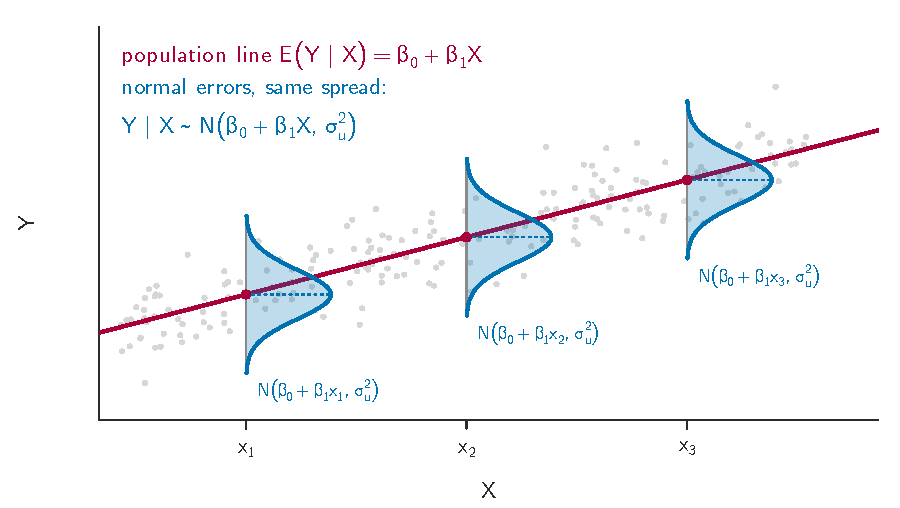
\includegraphics[height=0.82\textheight]{cond_normal.pdf}
\end{figure}

}



\frame{
\frametitle{Sampling Distribution for $\widehat{\beta}_1$}
\small
\vspace{-.5\baselineskip}
\begin{theorem}[Sampling Distribution of $\widehat{\beta}_1$]
Under Assumptions I--VI, conditional on $X$,
\vspace{-.5\baselineskip}
$$
\widehat{\beta}_1 \mid X \ \sim \ N\left(\beta_1, \var[\widehat{\beta}_1\mid X]\right)
$$
\vspace{-.5\baselineskip}
where
\vspace{-.5\baselineskip}
$$
\var[\hat{\beta}_1\mid X] \ = \ \frac{\sigma^2_u}{\sum_{i=1}^n(x_i - \bar{x})^2}
$$
\vspace{-.5\baselineskip}
which implies \pause
\vspace{-.5\baselineskip}
$$
\frac{\widehat{\beta}_1 - \beta_1}{\sqrt{\var[\hat{\beta}_1\mid X]}}
\ = \ \frac{\widehat{\beta}_1 - \beta_1}{SE(\hat\beta_1)} \ \sim \ N(0,1)
$$
\end{theorem}
\pause
\vspace{-.25\baselineskip}
\begin{proof}
\pause
\scriptsize{Given Assumptions I--VI, $\hat{\beta}_1$ is a linear combination of the i.i.d. normal random variables:
\vspace{-.5\baselineskip}
$$ \hat{\beta}_1  \ = \ \beta_1 + \sum_{i=1}^n \frac{(x_i - \bar{x})}{SST_x}u_i
\quad \text{where} \quad u_i \sim N(0,\sigma_u^2).
$$
\vspace{-\baselineskip}

Any linear combination of independent normals is \pause normal, \pause and we can transform/standardize any normal random variable into a standard normal by subtracting off its mean and dividing by its standard deviation.}
\end{proof}


}

\frame{
\frametitle{The t-Test for Single Population Parameters}
\small
\vspace{-.5\baselineskip}
\begin{itemize}
\item $SE[\hat{\beta}_1] =  \frac{\sigma_u}{\sqrt{ \sum_{i=1}^n(x_i - \bar{x})^2 }}$ involves the unknown population error variance $\sigma^2_u$
\item Replace $\sigma^2_u$ with its unbiased estimator $\hat{\sigma}^2_u = \frac{\sum_{i=1}^n \hat{u}_i^2}{n-2}$, and we obtain:
\end{itemize}
\vspace{-.5\baselineskip}
\begin{theorem}[Sampling Distribution of t-value]
Under Assumptions I--VI, the \alert{t-value} for $\beta_1$ has a $t$-distribution
with $n-2$ degrees of freedom:
$$
T \ \equiv \ \frac{\widehat{\beta}_1 - \beta_1}{\widehat{SE[\hat{\beta}_1]}} \ \sim \ \tau_{n-2}
$$
\end{theorem}\pause
\begin{proof}[Proof sketch]
\vspace{-.3\baselineskip}
\begin{itemize}
\item Given $X$, $\hat{\beta}_1 = \beta_1 + \frac{\sum_{i=1}^n (x_i-\bar{x})u_i}{SST_x}$ is a linear combination of normal errors, so $Z \equiv \frac{\hat{\beta}_1-\beta_1}{SE[\hat{\beta}_1]} \sim N(0,1)$
\item $Q \equiv \frac{(n-2)\hat{\sigma}^2_u}{\sigma^2_u} = \frac{\sum_{i=1}^n \hat{u}_i^2}{\sigma^2_u} \sim \chi^2_{n-2}$: the residuals lose two degrees of freedom to $\hat{\beta}_0$ and $\hat{\beta}_1$
\item Under normal errors, $\hat{\beta}_1$ is independent of the residuals (fitted values and residuals are orthogonal), so $Z$ and $Q$ are independent
\item Hence $T = \frac{Z}{\sqrt{Q/(n-2)}} \sim \tau_{n-2}$, by the definition of the $t$-distribution
\end{itemize}
\end{proof}
  % The logic is perfectly analogous to the t-value for the population mean --- because we are
% estimating the denominator, we need a distribution that has fatter tails than $N(0,1)$ to
% take into account the additional uncertainty. \\ \smallskip
% This time, $\hat\sigma^2_u$ contains two estimated parameters ($\hat\beta_0$ and $\hat\beta_1$)
% instead of one, hence the degrees of freedom $= n-2$. \\ \smallskip
% See Wooldridge's Appendix for a more formal proof.

}


\frame{
\frametitle{Using the t-Value as a Test Statistic}
\begin{footnotesize}
$$
T \ \equiv \ \frac{\widehat{\beta}_1 - c}{\widehat{SE}[\hat{\beta}_1]} \ \sim \ \tau_{n-2} \quad \text{if} \quad \beta_1 \ = \ c
$$
\begin{enumerate}
\item Assuming some \alert{null value} $c$ (e.g. $c=0$) and given the number of observations we know that the sampling distribution of this test statistic is $\tau_{n-2}$\medskip \pause
\item Given the null value, we can derive the probability that the value of our test statistics falls into a given interval:
$$
P\left(  -t_{\alpha/2}(n-2)   \le  T  \le  t_{\alpha/2}(n-2) \right)= 1- \alpha
$$\medskip \pause
\item Since we can also compute $\widehat{\beta}_1$ and $\widehat{SE}[\hat{\beta}_1]$ we can easily compute the realized t-value in our application.\medskip \pause
\item We can then check if the realized value is ``unusual'' given the known distribution of the test statistic.
    \end{enumerate}
\end{footnotesize}
%Assuming the null hypothesis is true, the test statistic (a random variable) has the following distribution:
%
%which we call a sampling distribution and more specifically a \alert{null distribution}. Notice that once we collect data, we will know all elements of this statistic.

}


\begin{frame}[t]
\frametitle{The Testing Workflow}
\small
\begin{enumerate}
\item Specify the \alert{null hypothesis} and \alert{alternative hypothesis}.
This is equivalent to setting the \alert{null value} c.
\end{enumerate}\medskip

Consider our regression example where $Y$: Trump's share of the two-party vote in 2024 (\%) and $X$: \% of adults 25 and older with a bachelor's degree, in the 50 states.\\\medskip

Suppose we are interested in testing $H_0: \beta_1 = c = 0$, versus $H_1: \beta_1 \ne c$. In words
we test whether \pause the population slope is zero.

\pause
\begin{itemize}
\item The null hypothesis is typically an assumed state of the world, or a strawman that we would like to knock down.\medskip\pause
\item The alternative hypothesis is typically a claim we would like to test. We call this particular alternative hypothesis a two-sided alternative, because evidence on either side of the hypothesized null value will help us to reject the null.\medskip \pause
    \item Notice we can use other values for $c$ than zero.
%\item We typically want strong evidence to reject the null, so we set a small probability of false rejection that we're comfortable with $\alpha$.\medskip
%\item Often, $\alpha = .05$, and yes, this is related to the $\alpha$ from the confidence interval section
\end{itemize}

\end{frame}

\begin{frame}[t]
\frametitle{The Testing Workflow}
\small
\begin{enumerate}
\item Specify the \alert{null hypothesis} and \alert{alternative hypothesis}
\item Specify the test level $\alpha$ ($=$ our tolerance for a type I error)
\end{enumerate}
{\small
Type I error $=$ \pause rejecting the null hypothesis when it is true; $\alpha$ is the probability of doing so that we accept
}
\medskip\pause

What is a good level of $\alpha$?\\\pause

\begin{itemize}
\item We typically want strong evidence to reject the null, so we set $\alpha$ to a small number like $.05$.
\end{itemize}

\end{frame}


\begin{frame}[t]
\frametitle{The Testing Workflow}
\small
\begin{columns} [t]
\begin{column}[]{6cm}
\begin{enumerate}
\item Specify the \alert{null hypothesis} and \alert{alternative hypothesis}.
\item Specify the test level $\alpha$.
\item Examine the \alert{null distribution} of the test statistic $T \sim \tau_{n-2}$
\end{enumerate}\medskip
We have 50 observations so the \alert{null distribution} is $T\sim \tau_{48}$
\end{column}
\begin{column}[]{5cm}

\begin{figure}[ht] \centering
        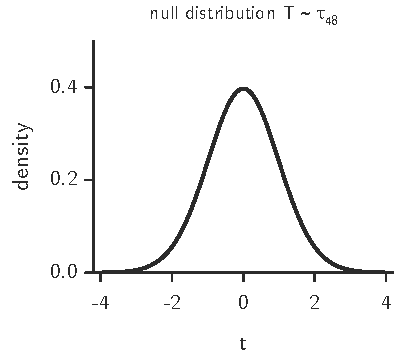
\includegraphics[width=\linewidth]{tdist_null.pdf}
\end{figure}

\end{column}
\end{columns}
\end{frame}


\begin{frame}[t]
\frametitle{The Testing Workflow}
\small
\begin{columns} [t]
\begin{column}[]{6cm}
\begin{enumerate}
\item Specify the \alert{null hypothesis} and \alert{alternative hypothesis}.
\item Specify the test level $\alpha$.
\item Examine the \alert{null distribution} of the test statistic
\item Determine the \alert{rejection region}
\end{enumerate}\medskip
At $\alpha=.05$ the \alert{critical value} $t_{\alpha/2}(48)$ is?
\pause \quad $2.01$\\\medskip
So we reject $H_0$ if: $$ |\mbox{our realized t-value}| \ > \ 2.01$$
\end{column}
\begin{column}[]{5cm}

\begin{figure}[ht] \centering
        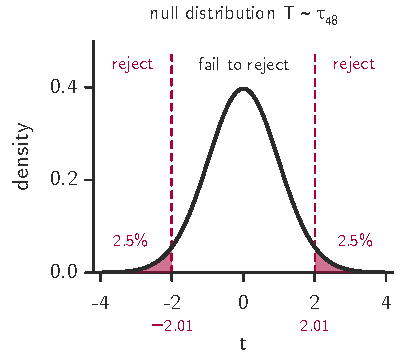
\includegraphics[width=\linewidth]{tdist_reject.pdf}
\end{figure}

\end{column}
\end{columns}
\end{frame}

\begin{frame}[t]
\frametitle{The Testing Workflow}
\small
\begin{columns} [t]
\begin{column}[]{6cm}
\begin{enumerate}
\item Specify the \alert{null hypothesis} and \alert{alternative hypothesis}.
\item Specify the test level $\alpha$.
\item Examine the \alert{null distribution} of the test statistic
\item Determine the \alert{rejection region}
\item Compute the \alert{observed} value of $T$ and
compare it to the critical value
\end{enumerate}\medskip
Here $\hat{\beta}_1=-1.4537$ and $\widehat{SE}(\hat{\beta}_1)=0.17376$ so  $T=\frac{-1.4537-0}{0.17376}=-8.37$. \\
So what do we conclude?\\\pause \medskip
We reject $H_0$ at the $.05$ level
\end{column}
\begin{column}[]{5cm}

\begin{figure}[ht] \centering
        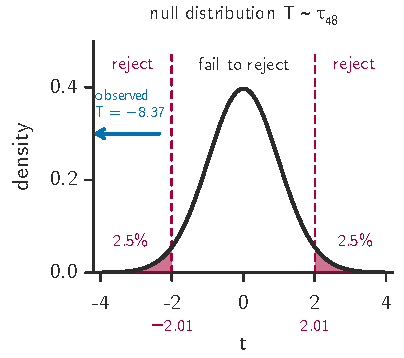
\includegraphics[width=\linewidth]{tdist_observed.pdf}
\end{figure}

\end{column}
\end{columns}
\end{frame}


\begin{frame}[fragile]
\frametitle{College Degrees and the 2024 Trump Vote, 50 States}
By default, R provides the t-values for the test against $H_0:
\beta = 0$ for slope and intercept

\medskip

{\spacingset{0.8}
\footnotesize
\begin{Verbatim}[frame=single, label=R Code, commandchars=\\\{\}]
> lm.out <- lm(trump ~ ba, data = states)
> summary(lm.out)

~~~~ output omitted ~~~~

Coefficients:
            Estimate Std. Error t value Pr(>|t|)
(Intercept) \textcolor{red}{102.8376}     \textcolor{red}{5.9818}  \textcolor{red}{17.192}  < 2e-16 ***
ba           \textcolor{red}{-1.4537}     \textcolor{red}{0.1738}  \textcolor{red}{-8.366}  6.2e-11 ***
---
Signif. codes:  0 '***' 0.001 '**' 0.01 '*' 0.05 '.' 0.1 ' ' 1

Residual standard error: 6.589 on 48 degrees of freedom
Multiple R-squared:  \textcolor{red}{0.5932},	Adjusted R-squared:  0.5847
F-statistic: 69.99 on 1 and 48 DF,  p-value: 6.199e-11
\end{Verbatim}
}
\end{frame}



\frame{
\frametitle{The p-value}
\small
\begin{columns} [c]
\begin{column}[]{6cm}
\begin{footnotesize}
\begin{itemize}
\item The $p$-value summarizes our evidence against $H_0$: it's the probability of observing a t-value (over repeated samples) at least as extreme as one we observe assuming that $H_0$ is true.\pause
\item $p$-value is $P(|T_0| > |T_{obs}|)$, the probability that the $t$-statistic under the null is larger \alert{in absolute value} than the observed $t$ value.\pause
\item If $p$-value $\leq \alpha$ we reject $H_0$ at the $\alpha$ level. It is therefore the smallest $\alpha$ for which we can reject $H_0$.
\end{itemize}\medskip
Given that $T_{obs}=-8.37$ will the p-value be small or large?\\\pause\medskip
p-value is $6.2\times 10^{-11}$ so we have strong evidence against $H_0$.
\end{footnotesize}
\end{column}
\begin{column}[]{5cm}

\begin{figure}[ht] \centering
        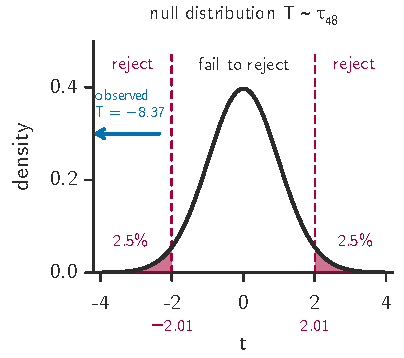
\includegraphics[width=\linewidth]{tdist_observed.pdf}
\end{figure}

\end{column}
\end{columns}
}

\begin{frame}[fragile]
\frametitle{College Degrees and the 2024 Trump Vote, 50 States}
{\spacingset{0.8}
\footnotesize
\begin{Verbatim}[frame=single, label=R Code, commandchars=\\\{\}]
> summary(lm.out)

~~~~ output omitted ~~~~

Coefficients:
            Estimate Std. Error t value Pr(>|t|)
(Intercept) \textcolor{red}{102.8376}     \textcolor{red}{5.9818}  \textcolor{red}{17.192}  \textcolor{red}{< 2e-16} ***
ba           \textcolor{red}{-1.4537}     \textcolor{red}{0.1738}  \textcolor{red}{-8.366}  \textcolor{red}{6.2e-11} ***
---
Signif. codes:  0 '***' 0.001 '**' 0.01 '*' 0.05 '.' 0.1 ' ' 1

Residual standard error: 6.589 on 48 degrees of freedom
Multiple R-squared:  \textcolor{red}{0.5932},	Adjusted R-squared:  0.5847
F-statistic: 69.99 on 1 and 48 DF,  p-value: 6.199e-11
\end{Verbatim}
}

\end{frame}


\frame{
\frametitle{A Null That Matters: Uniform Swing}
\small
Regress Trump's 2024 share on his 2020 share across the 50 states. Testing $\beta_1 = 0$ here tells us nothing new, because 2020 shares obviously predict 2024 shares. The interesting null is $H_0: \beta_1 = 1$. It says every state moved by the same number of points (a \alert{uniform swing}).
\vspace{-.1cm}
\begin{figure}[ht] \centering
        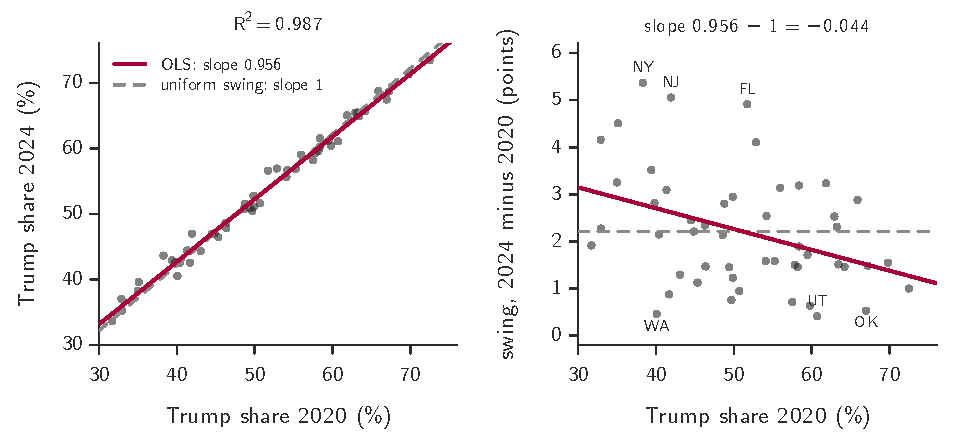
\includegraphics[height=0.52\textheight]{swing_scatter.pdf}
\end{figure}
\vspace{-.25cm}
{\footnotesize Dashed: the best line with slope 1 (every state moves 2.21 points). Solid: OLS. Right: the same two lines, with the swing (2024 minus 2020) on the vertical axis.}
\slidesource{MIT Election Data and Science Lab, 2020 and 2024 presidential returns by state. DC excluded.}
}

\begin{frame}[fragile]
\frametitle{A Null That Matters: Testing $H_0: \beta_1 = 1$}
{\spacingset{0.8}
\footnotesize
\begin{Verbatim}[frame=single, label=R Code, commandchars=\\\{\}]
> summary(lm(trump24 ~ trump20, data = states))
Coefficients:
            Estimate Std. Error t value Pr(>|t|)
(Intercept)  4.47307    0.81741   5.472 1.59e-06 ***
trump20      \textcolor{red}{0.95578}    \textcolor{red}{0.01564}  61.115  < 2e-16 ***
Residual standard error: 1.164 on 48 degrees of freedom
Multiple R-squared:  0.9873
\end{Verbatim}
}
\small
\begin{itemize}
\item R's t value (61.1) tests $\beta_1 = 0$. For $H_0: \beta_1 = 1$, set $c = 1$. \pause
Then $T=\frac{0.9558-1}{0.0156}=-2.83$. With 48 df, $p = .007$. We reject uniform swing at the $.05$ level.\pause
\item Every state moved toward Trump. Because $\hat\beta_1 < 1$, states that were more Republican in 2020 moved a little less. A state 10 points more Republican in 2020 has a fitted swing 0.44 points smaller.\pause
\item $R^2 = .987$ is not the point. It says 2020 shares predict 2024 shares almost perfectly. It does not tell us whether the slope is 1. The uniform-swing line fits almost as well ($R^2 = .985$).
\end{itemize}
\end{frame}


\frame{
\frametitle{One-Sided Versus Two-Sided Test}
\small
%\begin{columns} [c]
%\begin{column}[]{6cm}
%\begin{footnotesize}
\begin{itemize}
\item Using $H_0$: $\beta_1 = 0$ and $H_1$: $\beta_1 \neq 0$ is called a two-sided test because the null hypothesis can be rejected in both directions ($\beta_1 < 0$ and $\beta_1 >0$) \medskip
\item What is a one-sided test? \pause  $H_0$: $\beta_1 = 0$ and $H_1$: $\beta_1 < 0$ (say we were sure, before seeing the data, that states with more college graduates cannot give Trump a larger share). The null hypothesis can be rejected only in one direction.\medskip\pause
\item Given that we keep $\alpha=.05$ constant. What does this imply for the acceptance region? \pause All of the 5\% rejection region now sits in the lower tail, so the critical value is closer to zero: $-1.68$ instead of $\pm 2.01$ with 48 degrees of freedom. We reject more easily when $\hat\beta_1<0$, and never when $\hat\beta_1>0$.\medskip
    \item When is a one-sided test appropriate? \pause If the null can be wrong in only one direction and the other direction is completely inconceivable {\it a priori}. \pause
In other words, rarely in social sciences.
\end{itemize}
}

\frame{
\frametitle{Confidence Intervals}
\begin{footnotesize}
Suppose instead of a point estimator, we want to be more conservative, and specify an interval as our estimate for the location of the true slope $\beta_1$.\\\medskip This is straightforward now since we know the sampling distribution for our t-value:
$$
T = \frac{\widehat{\beta}_1 - \beta_1}{\widehat{SE}[\hat{\beta}_1]} \sim \tau_{n-2}
$$\pause
So we also know the probability that the value of our test statistics falls into a given interval:
\begin{align*}
P\left(  -t_{\alpha/2}(n-2)   \le     \frac{\widehat{\beta}_1 - \beta_1}{\widehat{SE}[\hat{\beta}_1]}  \le  t_{\alpha/2}(n-2) \right) &= 1- \alpha
\end{align*}\pause
In our example with $n=50$ and $\alpha=.05$ we know that:
\begin{align*}
P\left(  -2.01   \le     \frac{\widehat{\beta}_1 - \beta_1}{\widehat{SE}[\hat{\beta}_1]}  \le  2.01 \right) &= .95
\end{align*}
Recall: $t_{\alpha/2}(n-2)$ refers to the $100(1-\alpha/2)$ percentile in the $\tau_{n-2}$ distribution.
\end{footnotesize}
}

\frame{
\frametitle{Confidence Intervals}
\begin{footnotesize}
We rearrange:
\begin{align*}
P\left(  -t_{\alpha/2}(n-2)   \le     \frac{\widehat{\beta}_1 - \beta_1}{\widehat{SE}[\hat{\beta}_1]}  \le  t_{\alpha/2}(n-2) \right) &= 1- \alpha \\
P\left(   \widehat{\beta}_1-t_{\alpha/2}(n-2)\widehat{SE}[\hat{\beta}_1]  \le    \beta_1 \le  \widehat{\beta}_1 + t_{\alpha/2}(n-2)\widehat{SE}[\hat{\beta}_1]  \right) &= 1- \alpha
\end{align*}\pause

So we construct the confidence interval using:
$$
\hat{\beta}_1 \pm t_{\alpha/2}(n-2) \cdot \widehat{SE}[\hat{\beta}_1]
$$
\pause
In our example:
$$
-1.45 \pm 2.01\cdot 0.174\, \mbox{  so  }\, [-1.80\,,\,-1.10]
$$
Note that the random quantities in this statement are $\widehat{\beta}_1$ and $\widehat{SE}[\hat{\beta}_1]$. Therefore, once the data are observed, nothing else is random!\\\bigskip

In R: \texttt{confint(lm.out)}

\end{footnotesize}
}

\frame{
\frametitle{CIs Simulation Example}

Returning to the simulation example of Lecture 4-2, we can simulate the sampling distributions of the 95\% confidence intervals for $\beta_1$ and $\beta_0$
\vspace{-.0cm}
\begin{figure}[ht] \centering
        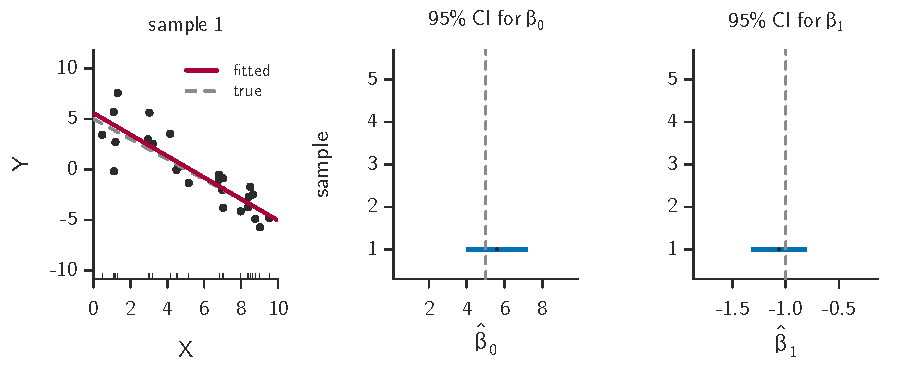
\includegraphics[height=0.68\textheight]{ci_sim_step1.pdf}
\end{figure}

}

\frame{
\frametitle{CIs Simulation Example}

Returning to the simulation example of Lecture 4-2, we can simulate the sampling distributions of the 95\% confidence intervals for $\beta_1$ and $\beta_0$
\vspace{-.0cm}
\begin{figure}[ht] \centering
        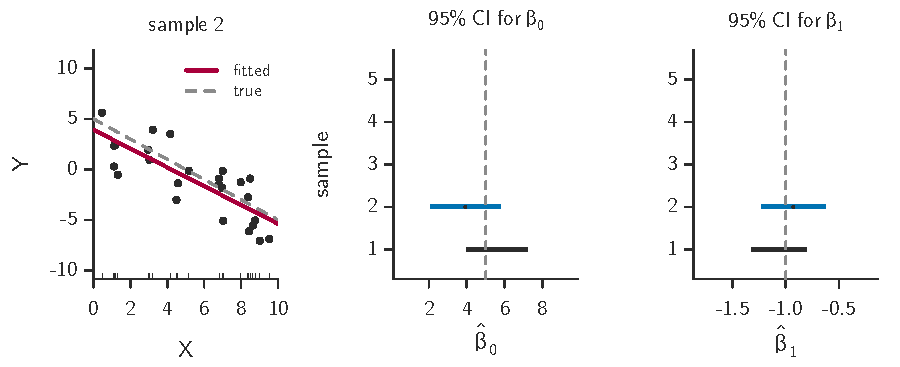
\includegraphics[height=0.68\textheight]{ci_sim_step2.pdf}
\end{figure}

}

\frame{
\frametitle{CIs Simulation Example}

\begin{figure}[ht] \centering
        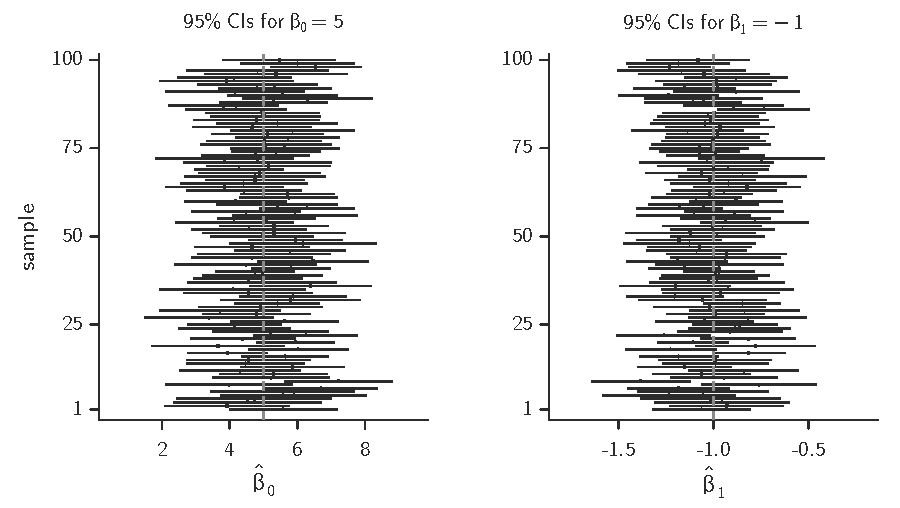
\includegraphics[height=0.81\textheight]{ci_sim_many.pdf}
\end{figure}

}

\frame{
\frametitle{CIs Simulation Example}

\begin{figure}[ht] \centering
        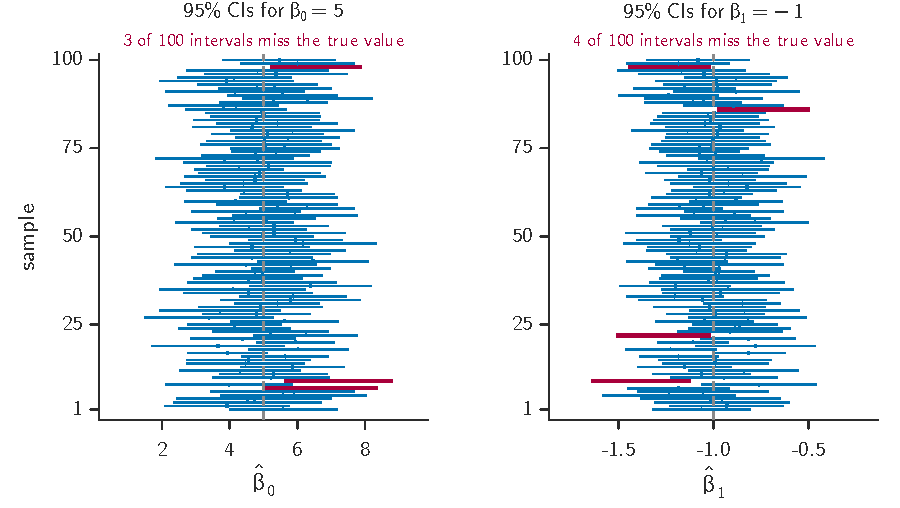
\includegraphics[height=0.81\textheight]{ci_sim_cover.pdf}
\end{figure}

}

\frame{
\frametitle{Testing with Confidence Intervals}

\begin{itemize}
\item Notice that the boundary of the upper critical region is $2.01$
\item Recall that this was the value of $t_{\alpha/2}(n-2)$ from our 95\% CI
\item This is not a coincidence, and it suggests a method for hypothesis testing with a confidence interval.
\end{itemize}
\vspace{.4cm}
\pause
Procedure:
\begin{enumerate}
\item Pick $H_0: \beta_1 = c$ and a significance level $\alpha$
\item Form a $100(1-\alpha) \%$ confidence interval
\item Reject the null if the CI doesn't contain $c$
\end{enumerate}\medskip
Our 95 \% CI was $[-1.80\,,\,-1.10]$ so we reject $H_0$: $\beta_1=0$ at the $\alpha=0.05$ level.

}

\subsection{Large Sample Inference}

\frame{
\frametitle{Large Sample Properties: Consistency}
\small
\begin{itemize}
  \item So far we have studied the \alert{small sample} properties of the OLS estimator, i.e.,
    how $(\hat\beta_0,\hat\beta_1)$ behaves {\it in repeated samples} of a given $n$.
  \item Now, we look at their \alert{large sample} properties, i.e.,
    how $(\hat\beta_0,\hat\beta_1)$ behaves {\it when $n \to \infty$}.
\end{itemize}
\pause
\begin{theorem}[Consistency of OLS Estimator]
Given Assumptions I--IV, the OLS estimator $\widehat{\beta}_1$ is consistent for $\beta_1$ as $n\rightarrow\infty$:$$
\plim_{n\to\infty} \widehat{\beta}_{1} = \beta_1
$$
\end{theorem}

\begin{proof}
\textbf{Worksheet Q1}
\end{proof}
}


\frame{
\frametitle{Large Sample Properties: Consistency}


%\begin{proof}
  % \begin{footnotesize}
% Similar to the unbiasedness proof:
% \begin{eqnarray*}
% \hat{\beta}_1 & = & \frac{\sum_{i=1}^n (x_i - \bar{x})y_i}{\sum_{i=1}^n (x_i - \bar{x})^2} = \beta_1 + \frac{\sum_i^n (x_i - \bar{x})u_i }{\sum_i^n (x_i - \bar{x})^2} \\ \pause
%  \mbox{plim } \widehat{\beta}_1 & = & \mbox{plim } \beta_1 + \mbox{plim } \frac{\sum_i^n (x_i - \bar{x})u_i }{\sum_i^n (x_i - \bar{x})^2} \quad \text{(Wooldridge C.3 Property i)} \\ \pause
%  & = & \beta_1 + \frac{\mbox{plim }\frac{1}{n}\sum_i^n (x_i - \bar{x})u_i }
%  {\mbox{plim }\frac{1}{n}\sum_i^n (x_i - \bar{x})^2} \quad \text{(Wooldridge C.3 Property iii)} \\ \pause
%  & = & \beta_1 + \frac{\cov[X,u]}{\var[X]} \quad \text{(by the law of large numbers)} \\ \pause
%  & = & \beta_1 \quad (\cov[X,u]=0 \ \text{and} \  \var[X]>0)
% \end{eqnarray*}

% \scriptsize{Technical aside: We divide denominator and numerator by $n$ to ensure that they have finite probability limits (otherwise they would increase without limit). Given finite limits we can apply the plim quotient rule: $\mbox{plim}\frac{A}{B}=\frac{\mbox{plim}\, A}{\mbox{plim}\, B}$}
% Now using a law of large numbers these sample quantities will converge in probability to the population quantities $n^{-1}\sum_i^n (x_i - \bar{x})u_i\stackrel{p}{\rightarrow}COV[X,u]$ and $n^{-1}\sum_i^n(x_i - \bar{x})^2\stackrel{p}{\rightarrow}\var[X]$ and therefore:
%$$\mbox{plim } \widehat{\beta}_{1,n} = \beta_1$$ given $COV[X,u]=0$ and $\var[X]>0$
%\end{footnotesize}
%\vspace{-.15in}
%\end{proof}

\begin{itemize}\itemsep1em
  \item Technical note: We can slightly relax Assumption IV:
$$ E[u|X]=0 \quad \text{(any function of $X$ is uncorrelated with $u$)} $$
 to its implication:
$$ \cov[u,X]=0  \quad \text{($X$ is uncorrelated with $u$)} $$
for consistency to hold (but not unbiasedness).\pause
  \item OLS is inconsistent (and biased) unless $\cov[X,u]=0$
  \item If $\cov[u,X]>0$ then asymptotic bias is upward; if $\cov[u,X]<0$ asymptotic bias is downwards
\end{itemize}

}


%\frame{
%\frametitle{Large Sample Properties: Consistency}

%\vspace{-.5cm}
%\begin{figure}[ht] \centering
%        \scalebox{.75}{\includegraphics{consistency.pdf}}
%\end{figure}
%Sampling distributions of $\hat\beta_1$, for sample sizes $n_1<n_2<n_3$
%}


\begin{frame}[t]
\frametitle{Large Sample Properties: Asymptotic Normality}
\small
\begin{itemize}
\item For statistical inference, we need to know the sampling distribution
of $\hat\beta$ when $n\to\infty$.
\end{itemize}
\begin{theorem}[Asymptotic Normality of OLS Estimator]
Given \alert{Assumptions I--V}, the OLS estimator $\widehat{\beta}_1$ is asymptotically normally distributed:
$$
\frac{\hat{\beta}_1 - \beta_1}{\widehat{SE}[\hat{\beta}_1]} \ \stackrel{approx.}{\sim} \ N(0,1)$$
where
$\widehat{SE}[\hat\beta_1] = \frac{\hat{\sigma}_{u}}{\sqrt{\sum_{i=1}^n (x_i - \bar{x})^2}}$ with the consistent estimator for the error variance:
$\hat{\sigma}^2_{u}=\frac{1}{n-2}\sum_{i=1}^n \hat{u}_i^2 \stackrel{p}{\rightarrow} \sigma^2_u$ (dividing by $n$ also works)
\end{theorem}

\bigskip\textbf{Worksheet Q2}
\end{frame}


\begin{frame}[t]
\frametitle{Large Sample Inference}
% \footnotesize
% \begin{proof}
% Proof is similar to the small-sample normality proof:
% \vspace{-.5\baselineskip}
% $$ \hat{\beta}_1  \ = \ \beta_1 + \sum_{i=1}^n \frac{(x_i - \bar{x})}{SST_x}u_i
% $$
% \vspace{-.5\baselineskip}
% $$ \sqrt{n}(\hat\beta_1 - \beta_1) \ = \
%  \frac{\sqrt{n}\cdot \frac{1}{n}\sum_{i=1}^n(x_i-\bar{x})u_i}{\frac{1}{n}\sum_{i=1}^n(x_i-\bar{x})^2}
% $$
% where the numerator converges in distribution to a normal random variable by CLT.
% Then, rearranging the terms, etc. gives you the right formula given in the theorem. \\ \smallskip
% For a more formal and detailed proof, see Wooldridge Appendix 5A.
% \end{proof}
% \pause
\begin{itemize}\itemsep1em
  \item We need homoskedasticity (Assumption V) for this result,
  but \alert{we do not need normality (Assumption VI)}.
  \item This result implies that \alert{asymptotically} our usual standard errors, t-values, p-values, and CIs remain valid even without the normality assumption!
 We just proceed as in the small sample case where we assume normality.
  \item It turns out that, given Assumptions I--V, the OLS asymptotic variance is also
  the lowest in class (asymptotic Gauss-Markov).
\end{itemize}
\end{frame}



\section{Interpreting OLS Coefficients}

\subsection{Predictive vs. Causal Interpretations}

\frame{
\frametitle{OLS Assumptions Summary}
\begin{center}
\olshierarchy{0}
\end{center}
}

\frame{
\frametitle{What Do the Regression Coefficients Mean Substantively?}
\begin{itemize}
\item So far, we have learned the \alert{statistical properties} of the OLS estimator
\medskip
\item However, these properties do not tell us what \alert{types of inference}
we can draw from the estimates
\medskip
\end{itemize}
\pause
Three types of inference:
\smallskip
	\begin{enumerate}
	\item Descriptive inference:
		\begin{itemize}
		\addtolength{\itemsep}{.25\baselineskip}
		\item Summarizing sample data by drawing the ``best fitting'' line
		\item No inference about the underlying population intended
		\item Assumption required: III (variation in $X$) only
		\end{itemize}
\pause
\medskip
	\item Predictive inference:
	    \begin{itemize}
		\addtolength{\itemsep}{.25\baselineskip}
	    \item Inference about a \alert{new observation} coming from the same population
	    \item Example: Wage ($Y$) and education ($X$): \\
	    ``What's my best guess about the wage of a new worker who only has high school
	    education?''
	    \item Assumptions required: III and II (random sampling)
	    \item Assumptions desired: I (linearity)
	    \end{itemize}
\end{enumerate}
}


\frame{
\frametitle{What Do the Regression Coefficients Mean Substantively?}
\begin{enumerate}
    \addtocounter{enumi}{2}
    \item Causal inference:
        \begin{itemize}
		\addtolength{\itemsep}{.25\baselineskip}
        \item Inference about \alert{counterfactuals}, i.e.
        hypothetical \alert{interventions} to the same units
        \item Example: Wage ($Y$) and education ($X$): \\
        ``What would my current wage be if I only had high school education?''
        \item Assumptions required (under the current framework):
        I, II, III and IV (zero conditional mean)
        \item In 450B, we will introduce a different framework which provides
        more nuanced views about \alert{causal identification assumptions}
        \end{itemize}	
\end{enumerate}
\pause
\begin{itemize}
\item Notice in the wage example, how the omission of unobserved ability from
the equation does or does not affect each type of inference
\pause
\medskip
\item Implications:
   \begin{itemize}
   \item When Assumptions I--IV are all satisfied, we can estimate the
   structural parameters $\beta$ without bias and thus make causal inference.
   \item However, we can make predictive inference even if some assumptions are violated.
   \end{itemize}
\end{itemize}
}


\frame{

\frametitle{OLS as a Best Linear Predictor}
\vspace{-.5\baselineskip}
\small
\begin{itemize}
\item Suppose that we want to predict the values of $Y$ given observed $X$ values
\item Suppose further that we've decided to {\it use} a linear predictor $\hat\beta_0
+ \hat\beta_1X$ (but not necessarily {\it assume} a true linear relationship in the population)
\pause
\item How to choose a good predictor? A popular criterion is \alert{mean squared error}:
$$
MSE \ = \ E\left[(Y - b_0 - b_1 X)^2\right]
$$
for a candidate line $b_0+b_1X$. The smaller a predictor makes $MSE$, the better.\pause
\item Now, note that the sample version of $MSE$ is $\frac{1}{n}\sum_{i=1}^n (y_i - b_0 - b_1 x_i)^2$\pause
\item Recall from Lecture 4-1 how we got the OLS estimator; we \textit{minimized} $\sum_{i=1}^n (y_i - \tilde\beta_0 - \tilde\beta_1 x_i)^2$ over $(\tilde\beta_0,\tilde\beta_1)$!\pause
\item This implies that OLS gives the best linear predictor \textit{in the sample}, and it estimates the population \alert{best linear predictor}, the line that minimizes $E[(Y-b_0-b_1X)^2]$\pause
\item Which assumptions did we use to get this result? \pause
 \begin{itemize}
  \item Needed: Assumptions II (random sampling) and III (variation in $X$)
  \item {\it Not} needed: Assumptions I (linearity) and IV (zero cond. mean)
 \end{itemize}
\item Note that if $E[Y|X]$ is linear (Assumptions I and IV), the population line is the \alert{best}, not just best linear, \alert{predictor}, so linearity is certainly desired
\end{itemize}
}




\frame{
\frametitle{OLS as an Estimator of Predicted Difference}
\small
\begin{itemize}
\item Recall the bias expression for $\hat\beta_1$ under Assumptions I--III (and not IV) from Lecture 4-2
for a binary explanatory variable:
$$ E[\hat\beta_1] \ = \ \beta_1 \ + \ \{ E[u\mid X=1] - E[u\mid X=0]\} $$
\item Suppose that the association between $u$ and $X$ is linear:
$$ u \ = \ \gamma_0 + \gamma_1X + \eta $$
where $E[\eta\mid X] = 0$ (Note that this is consistent with Assumption I)
\item Then, $\hat\beta_1$ estimates a different parameter $\beta_1^\ast$ without bias:
\begin{eqnarray*}
E[\hat{\beta}_1] &=& \beta_1 +\{E[u|X=1] - E[u|X=0]\} \\
  &=& \beta_1 +\{(\gamma_0 + \gamma_1\cdot 1 + 0) - (\gamma_0 + \gamma_1 \cdot 0 + 0)\}\\
  &=& \beta_1 +\gamma_1 \ \equiv \ \beta_1^{*}
\end{eqnarray*}
\item $\beta_1^\ast$ has a predictive interpretation, i.e.,
the expected difference between two randomly-drawn units
that happen to have $X=1$ and $X=0$ respectively

\end{itemize}

}



\subsection{Practical Advice}

\begin{frame}[fragile]
\frametitle{College Degrees and the 2024 Trump Vote, 50 States}
{\spacingset{0.8}
\footnotesize
\begin{Verbatim}[frame=single, label=R Code, commandchars=\\\{\}]
> summary(lm(trump ~ ba, data = states))

~~~~ output omitted ~~~~

Coefficients:
            Estimate Std. Error t value Pr(>|t|)
(Intercept) 102.8376     5.9818  17.192  < 2e-16 ***
\textcolor{red}{ba           -1.4537     0.1738  -8.366  6.2e-11 ***}
---
Signif. codes:  0 '***' 0.001 '**' 0.01 '*' 0.05 '.' 0.1 ' ' 1

Residual standard error: 6.589 on 48 degrees of freedom
Multiple R-squared:  0.5932,	Adjusted R-squared:  0.5847
F-statistic: 69.99 on 1 and 48 DF,  p-value: 6.199e-11
\end{Verbatim}
}
\begin{overprint}
\onslide<1|handout:0>
``The share of adults with a bachelor's degree is statistically significant ($p<0.001$)''
\onslide<2|handout:0>
``Trump's share of the vote decreases with the share of adults with a bachelor's degree ($p<0.001$)''
\onslide<3|handout:0>
\alert{Wrong:} ``A one percentage point increase in the share of adults with a bachelor's degree causes a $1.45$ percentage point decrease in Trump's share of the two-party vote ($p<0.001$).''
\onslide<4|handout:1>
``Across states, a share of adults with a bachelor's degree one percentage point higher is associated with a Trump share of the two-party vote $1.45$ percentage points lower ($p<0.001$).''
\end{overprint}

\end{frame}


\frame{
\frametitle{Ground Rules: Interpretation of the Slope}
\begin{enumerate}
  \item Give a short, but precise interpretation of the \alert{exact meaning} of the value of the slope coefficient referring to the concepts, units, direction, and magnitude.
\begin{itemize}
  \item Estimate suggests that one additional hour of reading the textbook is associated with 10 additional points on the exam.
\end{itemize}\medskip\pause

\item Do not resort to unwarranted causal language: Say ``predicts'', ``associated with'', ``expected difference'' or
``correlated with'' instead of ``causes'', ``leads'' or ``affects.'' \medskip\pause

\item Give a short, but precise interpretation of \alert{statistical
    significance}.
\medskip\pause
\item Give a short, but precise interpretation of \alert{practical significance}. You want to discuss the \alert{magnitude} of the slope in your particular application.
\end{enumerate}

}

\frame{
\frametitle{Reporting Statistical Significance}

\begin{itemize}
  \item A reasonable way to think about statistical significance is to think about the \alert{precision} of the estimates.\medskip
  \item If the slope is large substantively but just barely fails to reach conventional levels of significance it may still be interesting. \medskip
\item Examples:
\begin{itemize}
\item We reject the null hypothesis that the slope is zero at the $.05$ level.\medskip
\item The slope coefficient suggests that a one unit change in $X$ is associated with a 10 unit change in $Y$ (p$<.02$).\medskip
\item The slope coefficient is fairly precisely estimated, the 95 \% confidence interval ranging from 8 to 12. \medskip
    \end{itemize}
%\item Be careful when you say you ``accept'' $H_0$
\end{itemize}
}


\frame{
\frametitle{Reporting Substantive Significance}
\small
\begin{itemize}
  \item Statistical significance and substantive significance are not the same:  with a large enough sample size even truly microscopic differences can be statistically significant! \medskip
  \item To comment on substantive magnitude you should set up a ``plausible'' contrast keeping in mind (1) the distributions of variables and (2) the substantive context \medskip
\item Examples (the numbers in the first and third are made up for illustration):
\end{itemize}
\vspace{-.1in}
\begin{overprint}
\onslide<1|handout:0>
\begin{itemize}
\item[] Turnout on education: The slope estimate suggests that a high school dropout (10th percentile of the education distribution) on average has a $.3$ lower probability of voting compared to a college graduate (75th percentile of schooling).\\\smallskip The average probability of voting among HSDs is $.2$, so this corresponds to a $150$ \% increase for an average HSD.
\end{itemize}
\onslide<2|handout:0>
\begin{itemize}
\item[] Democracy on GDP (2024 data): Going from the 25th to the 75th percentile of GDP per capita (e.g.\ comparing the Republic of the Congo, \$6,153, and Romania, \$40,504) is associated with a $.20$ higher average electoral democracy index (V-Dem, 0 to 1). This moves a country from the 25th to about the 46th percentile of the democracy distribution.\\\smallskip For scale, the index is $.154$ at the 10th percentile (Burkina Faso, South Sudan), $.496$ at the median (Indonesia, Mexico) and $.840$ at the 90th (Austria, Canada, Iceland, US).
\end{itemize}
\onslide<3|handout:1>
\begin{itemize}
\item[] Earnings on Schooling: The slope estimate is \$4,000 per year of schooling. The standard deviation is $2.5$ years for schooling and \$50,000 for annual earnings. So a one standard deviation increase in schooling is associated with \$10,000 higher earnings, a $.2$ standard deviation increase.
    \end{itemize}
\end{overprint}
\only<2|handout:0>{\slidesource{V-Dem v16, electoral democracy index (\texttt{v2x\_polyarchy}), 179 countries; World Bank WDI, GDP per capita, PPP (2021 international \$), 168 of them. Regression of the index on log GDP per capita.}}
}

\subsection{Incorporating Nonlinearities using Log}

%\frame{
%\frametitle{Incorporating Nonlinearities}
%
%\begin{itemize}
%\item Notice that the ``linear'' in linear regression refers to \alert{linear in the parameters} not \alert{linear in the variables}.\\\bigskip
%\item We can incorporate non-linear relationships into our regression by first \alert{transforming} the variables\\\bigskip
%  \item A useful transformation when variables are positive and right-skewed is the (natural) logarithm\\\bigskip
%      \item Transformations that bring the distributions more in line with a normal distribution are also useful to stabilize the variance.
%\end{itemize}
%
%}


%\frame{
%\frametitle{Why the Log Transformation?}
%\small
%  The crucial property of natural logarithms? \pause $log(x_1)-log(x_0) \approx \pause \frac{(x_1-x_0)}{x_0}=\frac{\triangle x}{x_0}$.\\
%For \alert{small increments}, the difference of the logs of $x_1$ and $x_0$ approximates the percentage change in $x$ when going from the base level $x_0$ to the new level $x_1$   \\\bigskip
%  Now consider a linear model: $log(y)=\hat{\beta}_0 + \hat{\beta}_1 x$\\
%\pause
%$$
%\frac{\partial log(y)}{\partial(x)}=\beta_1 \, \Leftrightarrow \,\partial log(y) =\beta_1  \partial(x)
%$$\pause
%Notice$$
%\partial log(y) \approx \frac{\partial y}{ y} = \frac{\Delta y}{y} \mbox{ so } \partial log(y) \approx  \frac{\triangle y}{y} = \beta_1  \Delta x
%$$\pause
%And$$
%\% \Delta y = 100\beta_1  \Delta x
%$$
%Constant percentage change interpretation: A one unit increase in X is associated with a $100\cdot\beta_1$ \% increase in Y (works only for small increments).
%
%%  logs is the
%%  \begin{tabular}{c|c|c}
%%    \hline
%%    % after \\: \hline or \cline{col1-col2} \cline{col3-col4} ...
%%    Model & Equation & $\beta_1$ Interpretation \\
%%    \alert{Level-Level} & $Y=\beta_0 + \beta_1 X$ & $\partial Y=\beta_1\partial X $ \\
%%     \alert{Log-Level} & $log(Y)=\beta_0 + \beta_1 X$ & \%$\partial Y=100\beta_1\partial X $ \\
%%    \alert{Level-Log} & $Y=\beta_0 + \beta_1 log(X)$ & $\partial Y=(\beta_1/100)\%\partial X $ \\
%%    \alert{Log-Log} & $log(Y)=\beta_0 + \beta_1 log(X)$ & \%$\partial Y=\beta_1\%\partial X $ \\
%%    \hline
%%  \end{tabular}
%
%%  that the ``linear'' in linear regression refers to \alert{linear in the parameters} not \alert{linear in the variables}.\\\medskip
%%
%%
%%  \item Notice that Y and X are very right-skewed (we have a few large outliers) such that a linear summary is not terribly accurate
%%  \item In situations like this we can
%%  \item Hope is that linearity may be a better assumption on the transformed scale of the variables.
%
%}



\frame{
\frametitle{Incorporating Nonlinearities in $X$}

\begin{itemize}
\item The linear regression model {\it can} accommodate non-linearity in $X$
 (but not in $\beta$)
\item We do this by first \alert{transforming} $X$ appropriately \\\bigskip
  \item A useful transformation when variables are positive and right-skewed is the (natural) logarithm\\\bigskip
  \item The log transformation changes the interpretation of $\beta_1$:
    \smallskip
    \begin{itemize}
      \addtolength{\itemsep}{0.5\baselineskip}
      \item Regress $\log(Y)$ on $X$ $\longrightarrow$ $100\beta_1$ approximates the \alert{percent change} in $Y$ associated with a one-unit increase in $X$
      \item Regress $Y$ on $\log(X)$ $\longrightarrow$ $\beta_1/100$ approximates the change in $Y$ associated with a \alert{one percent increase} in $X$
      \item Note that these approximations work only for small changes
      \item In particular, they can fail for a dummy $D$ moving from 0 to 1 (Worksheet Q3)
    \end{itemize}
%\medskip
%  \item Other possible transformations: $X^2$, $\sqrt{X}$, $\log\l(\frac{Y}{1-Y}\r)$, etc.

\end{itemize}

}

\frame{
\frametitle{Example: Infant Mortality and National Income}
\small
\begin{figure}[ht] \centering
        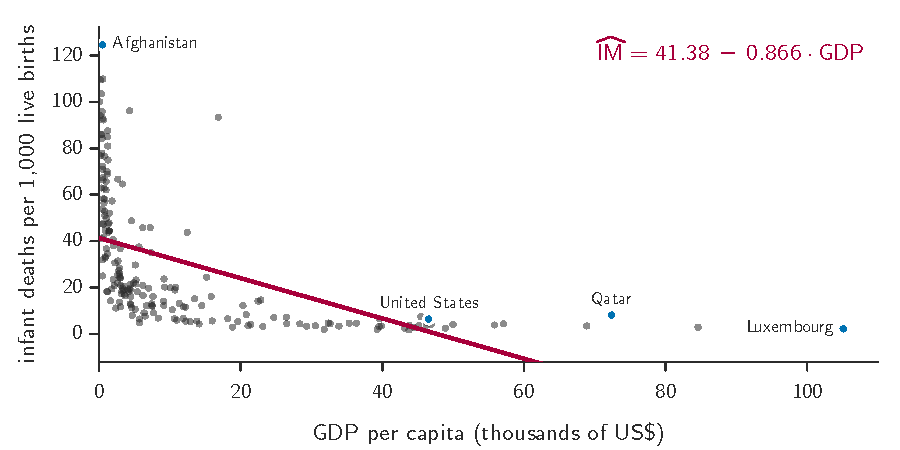
\includegraphics[height=0.61\textheight]{un_level.pdf}
\end{figure}
\vspace{-.15cm}
$\hat\beta_1 = -0.866$ $\longrightarrow$ \uncover<2->{An additional \$1,000 of GDP per capita predicts
$0.866$ fewer infant deaths per 1,000 live births on average}\\
\uncover<3->{But the line crosses zero at \$47,800, so it predicts negative infant mortality for the 8 countries richer than that.}
\slidesource{United Nations social indicators, mostly 2009--2011; 193 of the 213 countries and territories, those with both values (R package \texttt{carData}, data set \texttt{UN})}
}

\frame{
\frametitle{Infant Mortality (Scale in Levels)}
\begin{figure}[ht] \centering
        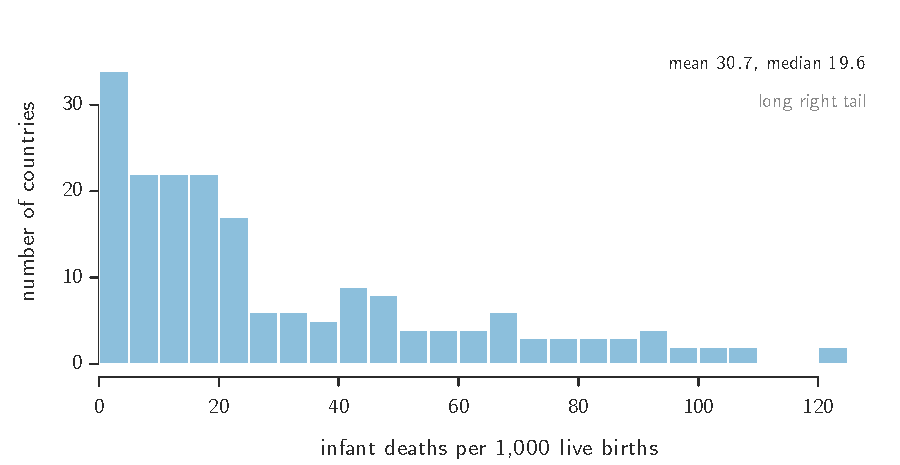
\includegraphics[height=0.73\textheight]{un_hist_level.pdf}
\end{figure}
\slidesource{United Nations social indicators, mostly 2009--2011; 193 of the 213 countries and territories, those with both values (R package \texttt{carData}, data set \texttt{UN})}
}

\frame{
\frametitle{Infant Mortality (Logarithmic Scale)}
\begin{figure}[ht] \centering
        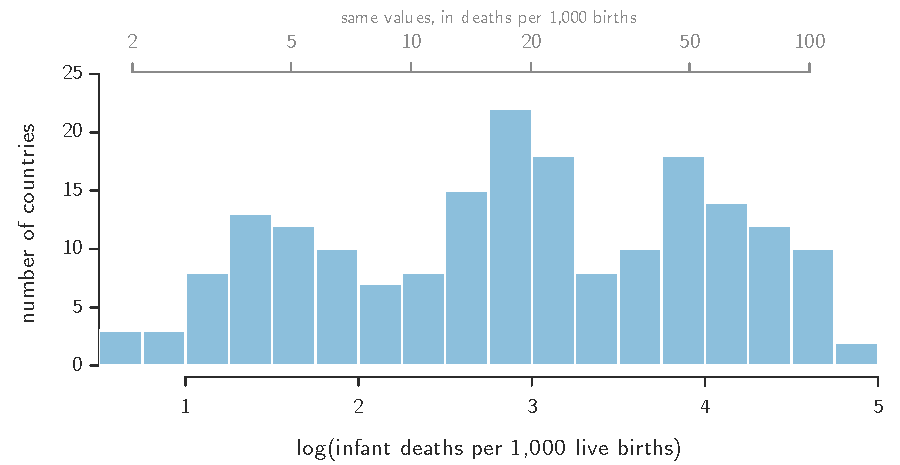
\includegraphics[height=0.73\textheight]{un_hist_log.pdf}
\end{figure}
\slidesource{United Nations social indicators, mostly 2009--2011; 193 of the 213 countries and territories, those with both values (R package \texttt{carData}, data set \texttt{UN})}

}


\frame{
\frametitle{Regression: Log-Level}
\small
\begin{figure}[ht] \centering
        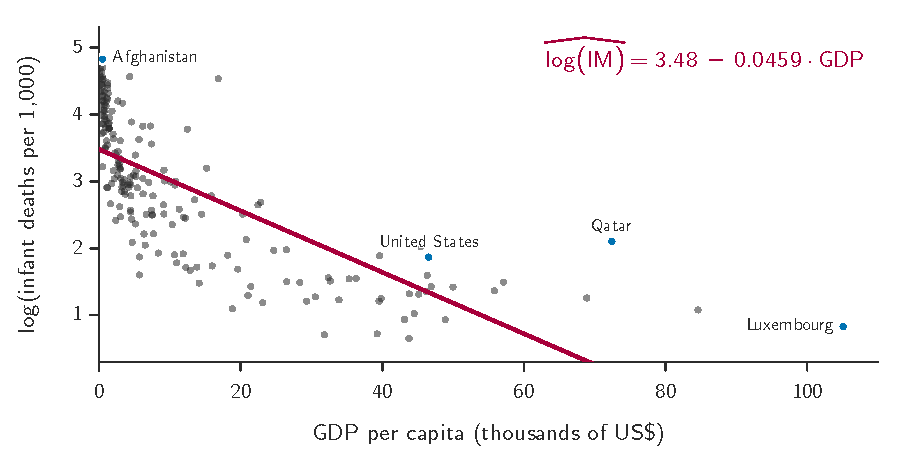
\includegraphics[height=0.65\textheight]{un_loglevel.pdf}
\end{figure}
\vspace{-.15cm}
$\hat\beta_1 = -0.0459$ $\longrightarrow$ \uncover<2->{An additional \$1,000 of GDP per capita predicts
an infant mortality rate about $4.6$ percent lower on average}
\slidesource{United Nations social indicators, mostly 2009--2011; 193 of the 213 countries and territories, those with both values (R package \texttt{carData}, data set \texttt{UN})}
}

\frame{
\frametitle{Regression: Log-Log}
\small
\begin{figure}[ht] \centering
        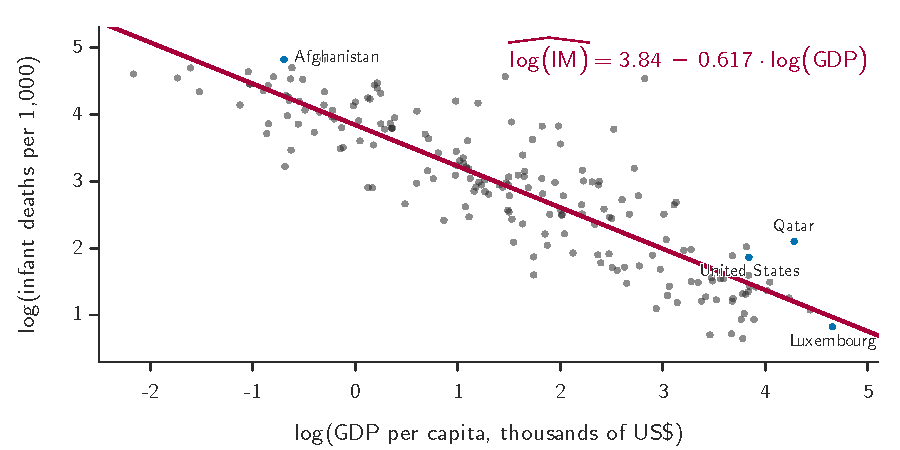
\includegraphics[height=0.65\textheight]{un_loglog.pdf}
\end{figure}
\vspace{-.15cm}
$\hat\beta_1 = -0.617$ $\longrightarrow$ \uncover<2->{A one percent increase in GDP per capita predicts
a $0.617$ percent decrease in infant mortality on average}
\slidesource{United Nations social indicators, mostly 2009--2011; 193 of the 213 countries and territories, those with both values (R package \texttt{carData}, data set \texttt{UN})}
}

\frame{
\frametitle{Four Most Commonly Used Models}

\begin{center}
  \begin{tabular}{c|c|c}
    \hline
    % after \\: \hline or \cline{col1-col2} \cline{col3-col4} ...
    Model & Equation & $\beta_1$ Interpretation \\
    \hline
    \alert{Level-Level} & $Y=\beta_0 + \beta_1 X$ & $\Delta Y=\beta_1\Delta X $ \\
     \alert{Log-Level} & $log(Y)=\beta_0 + \beta_1 X$ & \%$\Delta Y\approx 100\beta_1\Delta X $ \\
    \alert{Level-Log} & $Y=\beta_0 + \beta_1 log(X)$ & $\Delta Y\approx(\beta_1/100)\%\Delta X $ \\
    \alert{Log-Log} & $log(Y)=\beta_0 + \beta_1 log(X)$ & \%$\Delta Y\approx\beta_1\%\Delta X $ \\
    \hline
  \end{tabular}
\end{center}

\begin{itemize}\small
  \item \textbf{Level–Level:}  
  One additional year of education ($X$) is associated with an increase of $\beta_1$ thousand dollars in income ($Y$).  

  \item \textbf{Log–Level:}  
  One additional year of education ($X$) is associated with approximately $100\beta_1$ percent higher income ($Y$).  

  \item \textbf{Level–Log:}  
  A 1\% increase in population size ($X$) is associated with approximately a $\beta_1/100$ unit increase in government spending ($Y$).  

  \item \textbf{Log–Log:}  
  A 1\% increase in income ($X$) is associated with approximately a $\beta_1$\% increase in consumption ($Y$).  
\end{itemize}

%Other transformations (e.g. $\sqrt{x}$) are also sometimes used.

}

\frame{
\frametitle{Be Careful: Log-Level with binary $X$}

\textbf{Worksheet Q3}\\ \medskip

Consider $\log(Y)=\beta_0+\beta_1D + u$ with $D\in\{0,1\}$, assuming $D \perp u$.  \\

\begin{enumerate}\itemsep0.5em
    \item  Derive the exact percent change in $E[Y\mid D]$ when $D$ moves from $0$ to $1$.  
    \item  Explain why the rule “$100\cdot\beta_1\%$” is generally invalid here, and relate the sign and magnitude of the approximation error to $\beta_1$.  
    \item  For $\beta_1=0.30$, compute the exact percent change and the approximation error in percentage points.  
    \item  Find the value of $\beta_1>0$ above which the absolute approximation error exceeds $1$ percentage point.
\end{enumerate}
% Assume we have: $log(Y)=\beta_0 + \beta_1 \, D$ where $D$ is binary with values $1$ or $0$. Assume $\beta_1>.2$. What is the problem with saying that a one unit increase in $D$ is associated with a $\beta_1\, \cdot \,100$ percent change in $Y$?\\\bigskip \pause

% Log approximation is inaccurate for large changes like going from $D=1$ to $D=0$. Instead the percent change in Y when $D$ goes from $1$ to $0$ needs to be computed using:
% \begin{eqnarray}
% % \nonumber to remove numbering (before each equation)
% \nonumber
%    100(Y_{D=1}- Y_{D=0})/Y_{D=0} &=& 100((Y_{D=1}/Y_{D=0})-1) \\
% \nonumber   &=& 100((Y_{D=1}/Y_{D=0})-1) \\
% \nonumber   &=& 100(exp(\beta_1)-1)
% \end{eqnarray}
% Recall: $log(Y_{D=1})-log(Y_{D=0})=log(Y_{D=1}/Y_{D=0})=\beta_1$.\\\medskip
% A one unit change in $X$ (ie. going from 0 to 1) is associated with a
% $100(exp(\beta_1)-1)$ percent increase in $Y$.
}

\end{document}
